\documentclass[11pt]{report}
%---- defitions ----
\def\Author{Andreas Bock}
% <Add more defitions here>
%-------------------

%---- packages ----
\usepackage[]{amsmath}
\usepackage[english]{babel}
\usepackage[utf8]{inputenc}
\usepackage{graphicx}
\usepackage{moreverb}
\usepackage{enumitem}
\usepackage{amsthm}
\usepackage{amsmath}
\usepackage{amsfonts}
\usepackage{tcolorbox}
\usepackage{titlesec}
\usepackage{url}
\usepackage{verbatim}
\usepackage{mathrsfs}
\usepackage{upgreek}
\usepackage[
backend=biber,
style=alphabetic,
sorting=ynt
]{biblatex}
\addbibresource{main.bib}
\usepackage{xparse}
\usepackage{algorithm}
\usepackage{algpseudocode}
\usepackage{acro}
\usepackage{color}
\usepackage{bm}
\usepackage{listings}
\usepackage{nomencl}
\usepackage{soul}
\usepackage{hyperref}   
\usepackage{marginnote} 
\usepackage{tikz}
\usepackage{tocloft}
\usepackage{etoc}
\usepackage{xcolor}
\usepackage{dsfont}
\hypersetup{
    colorlinks,
    linkcolor={red!50!black},
    citecolor={blue!50!black},
    urlcolor={blue!80!black}
}
%---- settings ----
\usepackage[hmarginratio=1:1,margin=3.2cm,top=26mm,bottom=24mm]{geometry} % Document margins
% Set indentation
\setlength{\parindent}{0in}

% TOC stuff
\newlength\tocrulewidth
\setlength{\tocrulewidth}{1.5pt}
\parindent=0em
\etocsettocstyle{\rule{\linewidth}{\tocrulewidth}\vskip0.5\baselineskip}{\rule{\linewidth}{\tocrulewidth}}


\titleclass{\subsubsubsection}{straight}[\subsection]
\newcounter{subsubsubsection}[subsubsection]
\renewcommand\thesubsubsubsection{\thesubsubsection.\arabic{subsubsubsection}}
\renewcommand\theparagraph{\thesubsubsubsection.\arabic{paragraph}}
\renewcommand\thesubparagraph{\theparagraph.\arabic{subparagraph}}


% Theorems
\newtheorem{thm}{Theorem}
\newtheorem{mydef}{Definition}

% Font
\renewcommand*\rmdefault{ppl}
\renewcommand*{\marginfont}{\footnotesize}

% References & Nomenclature
\addto{\captionsenglish}{%
  \renewcommand{\bibname}{References}
  }
\renewcommand{\nomname}{Definitions and Nomenclature}
\makenomenclature
% ---------------------------------------------
% Theorems & Environments
% ---------------------------------------------
\newcounter{mythm}
\newcounter{mylem}
\newcounter{myrem}
\newcounter{myexa}
\newcounter{mypro}
\newcounter{mycol}
\newcounter{myass}
\newcounter{mysketch}
\newtheorem{theorem}[mythm]{Theorem}
\newtheorem{definition}[mydef]{Definition}
\newtheorem{remark}[myrem]{Remark}
\newtheorem{lemma}[mylem]{Lemma}
\newtheorem{example}[myexa]{Example}
\newtheorem{proposition}[mypro]{Proposition}
\newtheorem{corollary}[mycol]{Corollary}
\newtheorem{assumption}[myass]{Assumption}
\newtheorem{sketch}[mysketch]{Proof Sketch}
% Question & answers environment
\newcounter{question}[section]
\newenvironment{question}[1][]{\refstepcounter{question}\par\medskip
   \noindent \textbf{Question ~\thequestion. #1} \rmfamily}{\medskip}
\newenvironment{answer}{\par\medskip \itshape \paragraph{Answer to question ~\thequestion:}}{\hfill$\square$\medskip}
\newenvironment{research}{\itshape\color{purple}}{\medskip}

\newcommand{\andreas}[1]{{\itshape\color{purple} #1 }}
\newcommand{\mymarginnote}[1]{\marginnote{\itshape\color{olive} #1 }}
\newcommand{\todo}[1]{\textcolor{red}{\textit{ #1 }}}
%\newenvironment{komment}{\itshape Comment: }{\hfill$\clubsuit$}
%\newcommand{\komment}[1]{\begin{tcolorbox} \itshape Comment: \\
% #1 \end{tcolorbox}}

% Shorthands
\newcommand{\np}{$ \mathcal{NP} $}
\newcommand{\comm}[2]{{\sf \(\spadesuit\){\bf #1: }{\rm \sf #2}\(\spadesuit\)}}
\newcommand{\mcomm}[2]{\marginpar{\scriptsize \comm{#1}{#2}}}
\newcommand{\ab}[1]{\mcomm{AB}{#1}}
\newcommand{\simplex}{\textsc{Simplex} }
\newcommand{\Q}{\mathcal{Q} }
\newcommand{\Exp}[1]{\mathbb{E}\big[ #1 \big]}
\newcommand{\mL}{\mathcal{L} }
\newcommand{\bq}{\bm{q}}
\newcommand{\by}{\bm{y}}
\newcommand{\bx}{\bm{x}}
\newcommand{\bh}{\bm{h}}
\newcommand{\bW}{\bm{W}}
\newcommand{\bT}{\bm{T}}
\newcommand{\bX}{\bm{X}}
\newcommand{\R}{\mathbb{R}}
\newcommand{\Rm}{\mathbb{R}^m}
\newcommand{\half}{\frac{1}{2}}
\newcommand{\prob}[1]{\mathcal{P}\big[ #1 \big]}
\newcommand{\stone}{\underline{\emph{\bf Stage 1:}}}
\newcommand{\obs}{\underline{\emph{\bf Observe:}}}
\newcommand{\sttwo}{\underline{\emph{\bf Stage 2:}}}
\newcommand{\form}{\underline{\emph{\bf Formulate:}}}

\newcommand{\expect}[1]{\mathds{E}\big[ #1 \big]}
\newcommand{\covariance}[1]{\mathds{V}\big[ #1 \big]}

\newcommand{\cm}{\textsuperscript{\textcolor{red}{[Citation Missing]}}}
\newcommand{\transp}{^\top}
\newcommand{\invtransp}{^{-\top}}
\newcommand{\inv}{^{-1}}
\newcommand{\KL}[2]{\text{KL}{(#1, #2)}}
\newcommand{\statman}{\mathcal{H}}
\newcommand{\given}{\,|\,}
\newcommand{\trace}[1]{\textnormal{trace}\Big[ #1 \Big]}

% Inverse problems
\newcommand{\zk}{z_k}
\newcommand{\zkp}{z_{k+1}}
\newcommand{\zkpk}{z_{k+1|k}}
\newcommand{\zkpkp}{z_{k+1|k+1}}

\newcommand{\xk}{x_k}
\newcommand{\xkp}{x_{k+1}}
\newcommand{\xkpk}{x_{k+1|k}}
\newcommand{\xkpkp}{x_{k+1|k+1}}

\newcommand{\Xk}{X_k}
\newcommand{\Xkp}{X_{k+1}}
\newcommand{\Xkpk}{X_{k+1|k}}
\newcommand{\Xkpkp}{X_{k+1|k+1}}

\newcommand{\yk}{y_k}
\newcommand{\ykp}{y_{k+1}}
\newcommand{\ykpk}{y_{k+1|k}}
\newcommand{\ykpkp}{y_{k+1|k+1}}

\newcommand{\barXk}{\bar{X}_k}
\newcommand{\barXkp}{\bar{X}_{k+1}}
\newcommand{\barXkk}{\bar{X}_{k|k}}
\newcommand{\barXkpk}{\bar{X}_{k+1|k}}
\newcommand{\barXkpkp}{\bar{X}_{k+1|k+1}}

\newcommand{\hatXk}{\hat{X}_k}
\newcommand{\hatXkp}{\hat{X}_{k+1}}
\newcommand{\hatXkk}{\hat{X}_{k|k}}
\newcommand{\hatXkpk}{\hat{X}_{k+1|k}}
\newcommand{\hatXkpkp}{\hat{X}_{k+1|k+1}}

\newcommand{\hatxk}{\hat{x}_k}
\newcommand{\hatxkp}{\hat{x}_{k+1}}
\newcommand{\hatxkk}{\hat{x}_{k|k}}
\newcommand{\hatxkpk}{\hat{x}_{k+1|k}}
\newcommand{\hatxkpkp}{\hat{x}_{k+1|k+1}}

\newcommand{\Pkk}{P_{k|k}}
\newcommand{\Pkpk}{P_{k+1|k}}
\newcommand{\Pkpkp}{P_{k+1|k+1}}


\newcommand{\boldPkk}{\bm{P}_{k|k}}
\newcommand{\boldPkpk}{\bm{P}_{k+1|k}}
\newcommand{\boldPkpkp}{\bm{P}_{k+1|k+1}}

\newcommand{\ePkk}{P^E_{k|k}}
\newcommand{\ePkpk}{P^E_{k+1|k}}
\newcommand{\ePkpkp}{P^E_{k+1|k+1}}


%-------------------
\begin{document}
\title{Notes}% on Numerical Linear Algebra \& Functional Analysis}
\author{\Author}
\date{\today}
\maketitle
\tableofcontents

\chapter{Introduction}

\chapter{Principles}

\section{Notation}

A hat e.g. $\hat{x}$ means that this variable or data has some 
empirical nature or origin.

\section{What To Do About Training Data}

Typically all we have when we approach a problem that has some
statistical foundation is a finite collection of samples, say
$\hat{\xi}_i$, $i=1,\ldots,N$. These imply an empirical measure under some
assumption of their distribution.

\section{Maximum Likelihood Estimation}

Upon assuming some Gaussian data, we write the log-likehood
as follows:
\begin{align}
\hat{\mathcal{L}}(\mu, \Sigma\inv) & = -\frac{nN}{2}\log(2\pi)
+ \frac N2\log\det(\Sigma\inv) - \frac 12 \sum_{i=1}^N (\hat{\xi}_i - \mu)\transp\Sigma\inv (\hat{\xi}_i - \mu)\nonumber\\
& = -\frac{nN}{2}\log(2\pi)
+ \frac N2\log\det(\Sigma\inv)
- \trace{\hat{\Sigma}\Theta} - 
\frac 12  (\hat{\mu} - \mu)\transp\Sigma\inv (\hat{\mu} - \mu)
\label{eq:gaussian_log-likelihood}
\end{align}

The \emph{maximum likelihood estimator} $\Theta$ of the precision 
is given by:
\begin{align}
\Theta & = \arg\min_{\Theta\in\PD} \hat{\mathcal{L}}(\mu, \Theta)\nonumber\\
 & = \arg\min_{\Theta\in\PD} -\log\det(\Theta)
 + \trace{\hat{\Sigma} \Theta}.\label{eq:gaussian_log-likelihood:empirical}
\end{align}

The problem above is unbounded when $n>N$, since the SVD of the
sample covariance will decay to zero for some $i<n$, we can set
$\Theta$'s $i$\textsuperscript{th} singular value (indeed, its $i$ 
to $n$\textsuperscript{th}) to some $k>0$ and construct some
sequence of $k$'s such that 
\eqref{eq:gaussian_log-likelihood:empirical} is unbounded.
\chapter{Information Geometry}\label{ch:information_geometry}

\section{Basics}

\begin{itemize}
    \item Difference between KL and Wasserstein.
\end{itemize}
\chapter{Data Assimilation}\label{ch:filtering}
\localtableofcontents

\section{Introduction}

\section{Particle Filters}


\todo{Filter collapse}
\section{The Kalman Filter}

We are seeking to estimate a sequence of signal $x_t$, over some
time interval with steps $\delta t$, by only observing points $y_t$ that are assumed
to be in the range of some \emph{observation operator} plus added Gaussian noise.
That is, for each time point we seek an estimate $\hat{x}_{t+\delta t}$ of 
$x_{t+\delta t}$ provided cumulative information $y_t$. The (discrete time)
Kalman filter provides an unbiased estimate, indeed it provides the
\textbf{minimum variance unbiased estimator}:
\[
\hat{x}_{t+\delta t} := \arg\min_{x'} \expect{\|x' - x\|^2 \given y_t}.
\]

The Kalman filter results in closed form equations for $\hat{x}_{t+\delta t}$ based
on some assumptions about the evolution of $x$ and the relationship between
$x$ and $y$.

\iffalse
\begin{itemize}
    \item Singular evolutive extended Kalman filter (SEEK)
approximates the error covariance matrix by a singular low rank matrix, and makes correction only in those directions associated with the singular basis
    \item adding control to \eqref{eq:state_and_observation_equations}?
    \item filter inbreeding (P. Houtekamer and H. Mitchell. Data assimilation using an ensemble Kalman filter technique)
    \item Local ensemble transform Kalman filter
    \item 3D and 4D VaR
    \item Extensions \& Nonlinear Filtering
\end{itemize}

In this section, we describe the Kalman filter \cite{kalman1960new}, a predictive 
linear Gaussian filter whose the objective is generate a sequence of estimates of
a Gaussian random variable given a sequence of measurements. 
i.e. the posterior $\rho(X|Y)$ of a system i.e. the 
probability of $X\in\mathcal{X}$ given $y\in\mathcal{Y}$, via Bayes' rule:
\begin{equation}\label{bayesrule}
\rho(X|Y) \propto \rho(X)\rho(Y|X),
\end{equation}
for some prior information $\rho(X)\sim \mathcal{N}(\mu, C)$ about a state $X$ and likelihood $\rho(Y|X)$ of a prediction $Y|X\in\mathcal{Y}$.
\fi

\subsection{Assumptions}

We study the following linear system for $k=1,\ldots,K$:
\begin{subequations}\label{eq:state_and_observation_equations}
\begin{align}
& \xkp = F_k \xk + w_k, & \text{(state evolution equation)}\label{eq:KalmanState}\\
& y_k = H_k \xk + v_k, & \text{(observation or measurement equation)}\label{eq:KalmanMeasurement}
\end{align}
\end{subequations}
\mymarginnote{When $F_k=I$ for all $k$, this is referred to as a \emph{random walk forecast 
model.}}

where:
\begin{itemize}
    \item $x\in\mathcal{X}$ are the states that we want to recursively estimate.
    \item $F$ is a \emph{state transition model} (or \emph{state transition matrix} in finite dimension) applied to the previous state.
    %\item $B$ is a \emph{control-to-state} model which is applied to the control.
    \item $w\sim \mathcal{N}(0, Q_k)$ is process noise.
    \item $y_k\in\mathcal{Y}$ is an observation.
    \item $H:\mathcal{X}\rightarrow\mathcal{Y}$ is an \emph{observation} or \emph{measurement operator}.
    \item $v_k\sim \mathcal{N}(0, R_k)$ is observational noise.
\end{itemize}
The Kalman filter is a Markovian state model i.e. $\{ x_k\}_k$ is a Markovian process. This means 
the following assumptions hold for the mean zero noise variables:
\begin{align}
& \expect{w_k' w_l\transp} = Q_k \delta_{kl},\\
& \expect{v_k' v_l\transp} = R_k \delta_{kl}.
\end{align}
In other words, the state space noise $\{ x_k\}_k$ is white i.e. they are independent across $k$, as
well as having no correlation with the initial state, $x_0$. On top of that, we assume the following
about the initial state:
\begin{align}
& \expect{x_0} = \hat{x}_{0|0},\\
& \expect{(x_0-\hat{x}_{0|0})(x_0-\hat{x}_{0|0})\transp} = P_{0|0}.
\end{align}
\mymarginnote{Okay, get on with it!}
Based on these assumptions, we know that the state $x_k$ is Gaussian owing to the linearity assumption.

\subsection{Derivation}

We choose our prediction of the state at time $k+1$ provided all the time $k$ information as:
\begin{equation}\label{eq:hatxkpk_definition}
\hatxkpk = \expect{\xkp\given Y_k} := \expect{\xkp\given\{ z_i\}_{i=0}^k},
\end{equation}
giving rise to recursive expressions as we expand $\xkp$ via k\eqref{eq:KalmanState}.\\

The question is now: \textbf{how do update our prediction
when new information becomes available?} That is, how do we compute $\hatxkpkp$?
\mymarginnote{We don't want to forecast $k+2$ based on $\hatxkpk$ alone, we want to use
$\ykp$, got it!} \textbf{The goal is to determine a prediction $\hatxkpkp$ of the state $\xkp$
given information $Y_k := \{ y_i\}_{i=0}^k$ such that $\covariance{\hatxkpkp - \xkp}$ is minimised} 
in the \emph{minimum mean square error} (MMSE) sense.\\

Mathematically, we assume $\hatxkpkp = \pi (\hatxkpk, \ykp)$ for some $\pi$. We assume that $\pi$
is linear and write it as:
\begin{equation}\label{eq:hatxkpkp_MM_update}
\hatxkpkp = M \hatxkpk + M' \ykp,
\end{equation}
for some linear $M$ and $M'$ (eliding the dependency on $k$ to ease the notation). Let us examine
\eqref{eq:hatxkpkp_MM_update} and take its expectation (using \eqref{eq:KalmanMeasurement}):
\mymarginnote{$\hatxkp$ and $\hatxkpk$ are sometimes called the \emph{forecast} and \emph{analysis}
values of $x_{k+1}$.}
\begin{align*}
\expect{\hatxkpkp} & = \expect{M \hatxkpk + M' \ykp}\\
& = \expect{M\hatxkpk + M'  H_{k+1} \xkp + v_{k+1}}\\
& = \expect{M\hatxkpk + M'  H_{k+1} \xkp}\\
& = M\expect{\hatxkpk} + M'  H_{k+1} \expect{\xkp}\\
& = M\expect{\xkp} + M'  H_{k+1} \expect{\xkp},
\end{align*}
where the last equality holds by \eqref{eq:hatxkpk_definition}. Rewriting the expression
above we get:
\begin{equation}\label{eq:KalmanMMupdate_expectation}
\expect{\hatxkpkp} = \Big(M + M'  H_{k+1}\Big) \expect{\xkp}.    
\end{equation}
If we want the correction made to our forecast $\hatxkpk$ via \eqref{eq:hatxkpkp_MM_update} to be  
\emph{unbiased}, then the following equality \mymarginnote{We can't use $\xkp$ explicitly (because we don't have it), but
we can reason with it!} must hold:
\[
\expect{\hatxkpkp} = \expect{\xkp}.
\]
as well as \eqref{eq:KalmanMMupdate_expectation}, which means:
\[
M + M'  H_{k+1} = I.
\]
Rearranging, letting $M'=K_{k+1}$ and inserting this into \eqref{eq:hatxkpkp_MM_update}, the 
equation for $\hatxkpkp$ becomes:\mymarginnote{$K_{k+1}$ is called the \emph{Kalman gain}, and $\ykp - H_{k+1} \hatxkpk$ the \emph{innovation}.}
\begin{equation}\label{eq:hatxkpkp_final}
\hatxkpkp = \hatxkpk + K_{k+1} \big(\ykp - H_{k+1} \hatxkpk \big).
\end{equation}
\textbf{The question is now: how do you determine $K_{k+1}$?}. We can formulate the following
optimisation problem:
\begin{align*}
& \min_{K_{k+1}} \covariance{\hatxkpkp - \xkp\given Z_{k+1}}\\
= & \min_{K_{k+1}} \expect{(\hatxkpkp - \xkp)(\hatxkpkp - \xkp)\transp\given Z_{k+1}}\\
= & \min_{K_{k+1}} \trace{(\hatxkpkp - \xkp)(\hatxkpkp - \xkp)\transp}\\
= & \min_{K_{k+1}} \trace{\Pkpkp}\\
= & \min_{K_{k+1}} L(K_{k+1}).
\end{align*}

First, let's compute $\Pkpk$ because we will need it later on:
\begin{align}
\Pkpk & = \covariance{\hatxkpk - x_{k+1}\given Y_k} \\
& = \expect{(\hatxkpk - x_{k+1})(\hatxkpk - x_{k+1})\transp\given Y_k}\\
& = F_k\covariance{\hatxkk - x_k}F_k\transp + Q_k\\
& = F_k \Pkk F_k\transp + Q_k.
\end{align}
Next, computing the covariance matrix $\Pkpkp$ explicitly using \eqref{eq:hatxkpkp_final}:
\begin{align}
& \Pkpkp\\
= & \covariance{\hatxkpkp - x_{k+1}}\\
= & \covariance{\hatxkpk - x_{k+1} + K_{k+1}(\ykp - H_{k+1}\hatxkpk)}\\
= & \covariance{(I - K_{k+1} H_{k+1})\hatxkpk - x_{k+1} + K_{k+1}(H_{k+1}\xkp + v_{k+1})}\\
= & \covariance{(I - K_{k+1} H_{k+1})(\hatxkpk - x_{k+1}) + K_{k+1}v_{k+1}}\\
= & (I - K_{k+1} H_{k+1})\covariance{\hatxkpk - x_{k+1}}(I - K_{k+1} H_{k+1})\transp + \covariance{ K_{k+1}v_{k+1}}\text{\mymarginnote{\eqref{eq:JosephForm} is called the \emph{Joseph form}
of the update.}
}\\
= & (I - K_{k+1} H_{k+1})\Pkpk(I - K_{k+1} H_{k+1})\transp + K_{k+1}R_{k+1}K_{k+1}\transp.\label{eq:JosephForm}
\end{align} 
Equipped with this definition we inspect stationary points $\partial_K L = 0$ to finally 
arrive at a definition of the Kalman gain at each iterate $k>0$:
\begin{align*}
\partial_K L|_{K_{k+1}}= -2 (I - K_{k+1} H_{k+1}) \Pkpk H_{k+1}\transp + 2K_{k+1}R_{k+1}\transp = 0.
\end{align*}
Rearranging this expression we get:
\begin{equation}\label{eq:KalmanGain}
K_{k+1} = \Pkpk H_{k+1}\transp\big[H_{k+1}\Pkpk H_{k+1}\transp + R_{k+1}\big]\inv,
\end{equation}
which along with \eqref{eq:hatxkpkp_final} are the main equations of the Kalman filter.
\begin{remark}[Optimality]
Since $K_{k+1}$ is the minimiser of $L$, it is in this sense that the Kalman filter is \emph{optimal}
because it produces the state which minimises the mean squared error i.e. variance of the estimator.
Note that this statement does not depend on whether $x_0$, $w_k$ or $v_k$ are Gaussian.
\end{remark}
Knowing the expression for the gain we can simplify the Joseph form error covariance update
\eqref{eq:JosephForm}. Expanding this equation we get:
\begin{align*}
\Pkpkp & = \Pkpk - K_{k+1} H_{k+1}\Pkpk\\
& - \Pkpk H_{k+1}\transp K_{k+1}\transp + 
 K_{k+1}\big( H_{k+1}\Pkpk H_{k+1}\transp + R_{k+1})K_{k+1}\transp,
\end{align*}
and using \eqref{eq:KalmanGain} shows that the last two terms cancel, and we are left
with the folowing expression for the posterior estimate covariance matrix:
\begin{align}\label{eq:posterior_estimate_covariance}
\Pkpkp & = \Pkpk - K_{k+1} H_{k+1}\Pkpk = (I - K_{k+1} H_{k+1})\Pkpk.
\end{align}
We can also obtain a nice formula for its inverse, $\Pkpkp$. Indeed, inserting the expression
for the gain \eqref{eq:KalmanGain} in \eqref{eq:posterior_estimate_covariance}:
\[
\Pkpkp =  (I - \Pkpk H_{k+1}\transp\big[H_{k+1}\Pkpk H_{k+1}\transp + 
R_{k+1}\big]\inv H_{k+1})\Pkpk,
\]
and then using the Sherman-Woodbury-Morrison (SWM) identity:
\[
\Pkpkp = \big[\Pkpk\inv + H_{k+1}\transp R_{k+1}\inv H_{k+1}\big]\inv.
\]
By noting that $K_{k+1} = (\Pkpk - K_{k+1} H_{k+1} \Pkpk) H_{k+1} R_{k+1}\inv$ we can write 
\eqref{eq:hatxkpkp_final} in terms of $\Pkpkp$ (see also \cite{evensen2003ensemble,nino2015efficient}):
\begin{align*}
\hatxkpkp
& = \hatxkpk + K_{k+1} \big(\ykp - H_{k+1} \hatxkpk \big)\\
& = \hatxkpk - K_{k+1} H_{k+1} \hatxkpk + K_{k+1} \ykp\\
& = \hatxkpk - K_{k+1} H_{k+1} \hatxkpk + (\Pkpk - K_{k+1} H_{k+1} \Pkpk) H_{k+1} R_{k+1}\inv\ykp\\
& = (\Pkpk - K_{k+1} H_{k+1}\Pkpk)(\Pkpk\inv\hatxkpk + H_{k+1} R_{k+1}\inv\ykp)\\
& = (\Pkpk - \Pkpk H_{k+1}\transp\big[H_{k+1}\Pkpk H_{k+1}\transp + R_{k+1}\big]\inv H_{k+1}\Pkpk)\\
& \quad (\Pkpk\inv\hatxkpk + H_{k+1} R_{k+1}\inv\ykp)\\
& = \Pkpkp(\Pkpk\inv\hatxkpk + H_{k+1} R_{k+1}\inv\ykp).\qquad\quad \text{(SWM identity)}
\end{align*}
We have therefore demonstrated that we can write the update equations for the mean and covariance as:
\begin{align}
& \hatxkpkp = \Pkpkp(\Pkpk\inv\hatxkpk + H_{k+1}\transp R_{k+1}\inv\ykp)\\
& \Pkpkp\inv = \Pkpk\inv + H_{k+1}\transp R_{k+1}\inv H_{k+1} \label{eq:ForecastPosteriorSigma}.
\end{align}

\begin{algorithm}
\caption{Kalman Filter}\label{alg:kalman_filter}
\begin{algorithmic}
\Require $n \geq 0$
\Ensure $y = x^n$
\State $y \gets 1$
\State $X \gets x$
\State $N \gets n$
\While{$N \neq 0$}
spot\If{$N$ is even}
    \State $X \gets X \times X$
    \State $N \gets \frac{N}{2}$  \Comment{This is a comment}
\ElsIf{$N$ is odd}
    \State $y \gets y \times X$
    \State $N \gets N - 1$
\EndIf
\EndWhile
\end{algorithmic}
\end{algorithm}

\begin{question}
What is the computational complexity of the Kalman filter (per iteration)?
\end{question}
\begin{answer}
Recall that the state vector has dimension $n$ and the observation space has dimension $m$.
Owing to the presence of matrix multiplication and inverses, the most na\"ive complexity of
algorithm \ref{alg:kalman_filter} is $O(m^3 + n^3)$.
See also \cite{saibaba2015fast}.
\end{answer}

The forecast covariance, $\Pkpk$, is typically unknown and must be estimated from the forecast
itself. However, if the dimension $n$ of the (unobserved) state or $m$ of the observations is very
large, then the inverses of $\Pkpk$ (of size $n\times n$) or the $m\times m$ inverse matrix
in \eqref{eq:KalmanGain} become costly. 

\begin{example}[Pendulum tracking]
For instance, think of a pendulum and how the observations are in 2D, but the state contains
approximations of higher order moments like derivatives in addition to it. As you keep adding Taylor
terms, the dimension of the state increases.
\end{example}

\subsection{Shortcomings}\label{sec:shortcomings_and_overview}

The success of the Kalman filter has motivated numerous extensions seeking to overcome
some of the shortcomings that the assumptions of the Kalman filter rely on. The two
principal concerns that these extensions try to overcome are scalability and linearity.\\

\textbf{High dimensionality}\\
The cubic scaling in $n$ is prohibitive when performing data assimilation for high-dimensional
systems. As we shall see in the next section, an \emph{ensemble} can be maintained that reduces
this scaling at the cost of some inaccuracies in the estimation. Furthermore, the scaling in $m$ can
also be remedied by diligent use of matrix identities, reducing the scaling to $n + m$ times a
quadratic term in the dimension of the so-called ensemble approximation.\\

\textbf{Linearity}\\
Second, the assumption that the state and observation operators are linear are not valid for
many real applications e.g. numerical weather prediction (NWP). There are linearisation procedures
and other avenues that have been explored in order to - rather successfully - apply the Kalman
filter idea to nonlinear systems.\\

The EKF just linearises nonlinear forward maps.

\section{The Ensemble Kalman Filter}

The EnKF is a Monte Carlo data assimilation \cite{reich2015probabilistic} algorithm dating back to 1994 \cite{evensen1994sequential} of the Kalman filter. An excellent introduction to the EnKF can be found in \cite{katzfuss2016understanding}. Its main motivation is to circumvent one of
the main drawbacks of the Kalman filter when $n$ is large. We refer to \cite{roth2017ensemble} for a signal processing perspective on the EnKF. Indeed, the Kalman filter propagates the
forecast covariance over its iterations, so the size of $\Pkpk$ obviously scales quadratically in
$n$. This is prohibitive, so instead of propagating our mean and covariance through the filter, we 
keep track of $N_E$ different states of the system and propagate them and \emph{then} compute their 
sample covariances. That is, instead
\mymarginnote{Right, so $N_E<<n$? I'm sure that doesn't cause any issues...}
of computing with an $n$-dimensional estimate and its $n\times n$ covariance matrix, we instead
keep track of $N_E$ different state vectors of size $n$, and via the state equation, estimate a 
covariance matrix based on this. In the Kalman filter, you advance the \emph{whole} covariance
forward as the steps progress cf. equation \eqref{eq:covariance:I-KHP}. We simply estimate it in the
EnKF using $N_E$ state vectors (resulting in total storage of $N_E \times n$), and while the he 
resulting  covariance matrix will also have dimension $n\times n$ \emph{but we never explicitly
compute it}!\\

Mathematically, the EnKF instead computes at each step $k$ sample statistics from a collection, or
\emph{ensemble}, $\hatXkk = \{\hatXkk^i\}_{i=1}^{N_E}$, of $N_E$ state vectors taking values in
$\mathcal{X}$ equipped with an inner product $\langle\cdot, \cdot\rangle_\mathcal{X}$.
We consider the following prior forecast, for iterations $k\geq 1$ and ensemble members
$i=1,\ldots,N_E$:
\begin{align}\label{eq:enkf_forecasting}
& \hatXkpk^i = F_{k+1} \hatXkk^i  + w_{k+1}^i, & w_{k+1}^i\sim \mathcal{N}(0, Q_k).
%& Y_k^i = H_k \Xk + v_k^i, & v_k^i \sim \mathcal{N}(0, R_k),
\end{align}

\begin{remark}
\eqref{eq:enkf_forecasting} is called \emph{stochastic} EnKF due to the added noise.\\
\end{remark}

For such a forecast ensemble we compute the \emph{sample mean forecast} $\barXkpk$ and write the action of the \emph{sample forecast covariance error} $\ePkpk$:
\begin{align}
& \barXkpk := \frac{1}{N_E}\sum_{i=1}^{N_E} \hatXkpk^i,\label{enkf_approximations:X}\\
& \ePkpk[\cdot] := \frac{1}{N_E-1}\sum_{i=1}^{N_E} (\Xkpk^i-\bar{X}_k)\langle \hatXkpk^i-\bar{X}_k,\cdot\rangle_\mathcal{X}\label{enkf_approximations:COV}.
\end{align}
Using the EnKF approximations \eqref{enkf_approximations:X} and \eqref{enkf_approximations:COV}
we write the \emph{ensemble} Kalman gain and ensemble update as follows:
\begin{subequations}\label{eq:naive_enkf_update}
\begin{align}
& K_{k+1}^E = \ePkpk H_{k+1}\transp\big[ H_{k+1}\ePkpk H_{k+1}\transp + R_{k+1}\big]\inv,\label{eq:kalman_update}\\
& \hatXkpkp^i = \hatXkpk^i + K_{k+1}^E (\ykp - H_{k+1} \hatXkpk^i),\qquad i=1,\ldots,N_E.\label{eq:ensemble_update}
\end{align}
\end{subequations}
where the latter can be compute when a new observation $\ykp$ is available. Note that 
\eqref{eq:ensemble_update} parallelizes across the ensemble members. The trade-off here is that we
must evolve a system of equations.\\

\begin{remark}[Nonlinearity]
The EnKF is used across many fields for highly nonlinear systems (i.e. $F$ and $H$ are generic operators),
breaking with the original assumptions of the Kalman filter. Despite this, the success of the EnKF can be boiled down the the following quote:\\

\textit{"It is an embodiment of the principle that an approximate solution to the right
problem is worth more than a precise solution to the wrong
problem."} \cite{katzfuss2016understanding}.\\

The EnKF update is in fact also a nonlinear system owing to the dependence of the Kalman gain on the ensemble itself via the sample statistics, breaking with the Gaussian assumption of the ensemble. In the limit of large ensembles the EnKF can be shown to converge to the Kalman filter \cite{le2009large,mandel2011convergence}.
\end{remark}

\begin{remark}[Choice of initial ensemble]
Here, $X_0$ is the initial ensemble.
\end{remark}

\subsection{Complexity Analysis}
As it stands, \eqref{eq:naive_enkf_update} can be improved because a Cholesky factorisation of order
$O(m^3)$ is needed to compute the inverse in \eqref{eq:kalman_update}. We can reduce this by some linear
algebra. Writing \eqref{enkf_approximations:COV} in matrix form:
\[
\ePkpk = \frac{1}{N_E-1} X^E_{k+1|k} (X^E_{k+1|k})\transp,
\]
where $X^E_{k+1|k} = \Xkpk - \barXkpk$ and expanding this expression in \eqref{eq:kalman_update}:
\begin{align*}
\hatXkpkp^i & = \hatXkpk^i + K_{k+1}^E (\ykp - H_{k+1} \hatXkpk^i),\\
& = \hatXkpk^i + \ePkpk H_{k+1}\transp\big[H_{k+1}\ePkpk H_{k+1}\transp + R_{k+1}\big]\inv (\ykp - H_{k+1} \hatXkpk^i),\\
& = \hatXkpk^i + \frac{1}{N_E-1}X^E_{k+1|k} (X^E_{k+1|k})\transp H_{k+1}\transp\\
& \qquad\quad \big[H_{k+1}\frac{1}{N_E-1}X^E_{k+1|k} (X^E_{k+1|k})\transp H_{k+1}\transp + R_{k+1}\big]\inv (\ykp - H_{k+1} \hatXkpk^i),\\
& = \hatXkpk^i + \frac{1}{N_E-1}X^E_{k+1|k} A\transp \big[\frac{1}{N_E-1}A A\transp + R_{k+1}\big]\inv (\ykp - H_{k+1} \hatXkpk^i),
\end{align*}
where $A = H_{k+1}X^E_{k+1|k}$. Applying the SWM identity to the inverse gives us
\[
\big[\frac{1}{N_E-1}A A\transp + R_{k+1}\big]\inv =
R_{k+1}\inv - \frac{1}{N_E-1} R_{k+1}\inv  A\big[I + \frac{1}{N_E-1}A\transp R_{k+1}\inv  A\big]\inv A\transp R_{k+1}\inv.
\]
Following \cite{mandel2006efficient}, we can therefore assemble $\hatXkpkp$ as:
\begin{subequations}\label{eq:efficient_update}
\begin{align}
\hatXkpkp^i & = \hatXkpk^i + \frac{1}{N_E-1}X^E_{k+1|k} Z, & O(nN_E^2)\label{eq:efficient_update:1}\\
Z & = A\transp L, & O(m N_E^2)\label{eq:efficient_update:2}\\
L & = R_{k+1}\inv - \frac{1}{N_E-1} R_{k+1}\inv A W, & O(m N_E^2)\label{eq:efficient_update:3}\\
W & = S\inv Z', & O(N_E^3) \label{eq:efficient_update:4}\\
S & = I + \frac{1}{N_E-1}A\transp R_{k+1}\inv A & \label{eq:efficient_update:5}\\
Z' & = A\transp R_{k+1}\inv (\ykp - H_{k+1} \hatXkpk^i), & O(m N_E^2)\label{eq:efficient_update:6}\\
A & = H_{k+1} X^E_{k+1|k}. & O(m N_E)\label{eq:efficient_update:7}
\end{align}
\end{subequations}
Consequently, the total complexity of \eqref{eq:efficient_update} is $O(N_E^2 (m + n)
+ N_E^3)$. Note that it is assumed in \eqref{eq:efficient_update:7} that an evaluation
$h(x)$ of the observation operator is $O(m)$ (so it's not a full $O(mn N_E)$ operation
to compute $A$).

\mymarginnote{This might be a good exam question!}

%EnKF is also robust to nonlinear systems (be it $H$, $M$ or both). It is a consequence
%of \emph{linear Bayesian estimation}, where...
%\todo{This}
%\todo{Mention that enkf also reduces ensemble spread via: \tcite{sakov2008deterministic}!}

\begin{remark}[Literature \& Perspective]
\end{remark}

\subsection{Effect of Monte Carlo Approximation}

\todo{Cite Ruth's MSc thesis here}

Since $P$ is a Monte Carlo approximation of the full covariance, small ensembles significantly
\emph{undersample} the true statistics of the filter. This causes a variety of issues:
\begin{itemize}
    \item Spurious correlations between elements of the state vector (e.g. different
    grid points in a discretisation of a domain) that represent unnatural or unphysical behaviour,
    degrading the overall quality of the sample covariance.
    \item Underestimate background covariance,
    \item Filter inbreeding,
    \item Filter divergence:
    \item Full rank MCMC etc.
\end{itemize}

One of the most successful ensemble Kalman filter (EnKF) formulations is the local
ensemble transform Kalman filter (LETKF) in which the impact of spurious analysis
correlations is avoided by making use of local domain analyses. In this context, every
model component is surrounded by a box of a prescribed radius, and then the
assimilation is performed within every local box. In this case the background error
correlations are provided by the local ensemble covariance matrix. The local analyses
are mapped back onto the global domain to obtain the global analysis state.

\section{Variants}

\subsubsection{Square Root Filters}

\todo{Nonuniqueness of sqrt filters?}

% SQUARE ROOT HERE
Deterministic forecasts also exist i.e. where Square-root filters do not compute
\eqref{eq:enkf_forecasting} in practice. Instead,\\

Square root filters rely on the observation that the root of the prior forecast matrix
$\Pkpk$ can be decomposed:
\[
\Pkpk = L L'.
\]
Letting $D:=H_{k+1}\Pkpk H_{k+1}\transp + R_{k+1}$, then \eqref{eq:ForecastPosteriorSigma} 
can be written as ...

\subsubsection{Unscented Kalman Filter}

\cite{julier1997new}

\section{Variational Methods}

\todo{Difference between Bayesian and variational methods}

\subsection{Variational Kalman Filter (VKF)} 

Was introduced in Auvinen et al (2009).\\

There is also a smoothing variant: the Variational Kalman Smoother iterates VKF over the entire
assimilation window but instead of observations it uses the
analysis from the previous iteration cycle as the observations.

\subsection{Variational Ensemble Kalman Filter (VEnKF)}

Introduced first in Solonen (2012) 
\section{4D Var}

\textbf{Variational:} means...\\

Kalman filters work well but they have a characteristic defect
in that, unlike 4DVar, they leave behind discontinuous model
trajectories that do not correspond to physically consistent and
continuous model states.

Assimilation is largely on the following form:\\
\[
J(x_a) = (x_a-x_f)\transp B\inv (x_a - x_f) + (H(x_a)- y)\transp R\inv (H(x_a)-y).
\]

Satellite radiances
\section{Ensemble Kalman Inversion}

While the standard EnKF is typically used as an inference tool it has also been proposed as a way to 
solve general class inverse problems
\cite{oliver2008inverse,iglesias2013ensemble,iglesias2016regularizing,chada2018parameterizations,schillings2017analysis}, supported by a wide array of numerical evidence in particular for data assimilation in atmospheric science (see e.g. \cite{schneider2017earth} and its bibliography). We briefly outline the steps of an iterative EnKF method for a Bayesian inverse problem roughly on the form \emph{given $y$, find the $x$ such that $y \approx H[x]$}, where $H$ now is a specified uncertainty-to-state operator. {The key in this approach is that the term $y - H \Xk$ in \eqref{ensembleupdate} now represents the misfit that we want to minimize (modulo possible added noise).
\begin{itemize}
    \item Denote by $X_0 = \{X_0^i\}_{i=1}^{N_E}$ the initial ensemble.
    \item For $k=0,\ldots,n-1$:
\begin{enumerate}
    \item Propagate the ensemble through the uncertainty-to-state operator:
    \begin{align} Y_k := \{Y_k^i\}_{i=1}^{N_E} = \{H[\Xk] + v_k^i\}_{i=1}^{N_E}, \quad v_i \in \mathcal{N}(0, R_k),\; i=1,\ldots,N_E.\label{eq:Yk}
    \end{align}
    \item Compute $K_{k+1}^E$ using $X_k$ and $Y^k$ in \eqref{enkf_approximations:X} and \eqref{enkf_approximations:COV}.
    \item Update the ensemble: \[ X_{k+1} = X_k + K_{k+1}^E (y - Y^k),\] where these operations are understood element-wise across the ensemble.
\end{enumerate}
\end{itemize}
}
% Link with existing methods
Under certain assumptions on the linearity of $H$ and the covariance operators $C$ and $R$ it can be shown \cite[Section 2.6]{iglesias2013ensemble} that the iterative EnKF approximates, without the use of derivatives, a solution to the Tikhonov-Philips \cite{vogel2002computational} regularised functional:
\[
x\mapsto \| y - H x \|_\mathcal{Y}^2 + \| x - \bar{x} \|_\mathcal{X}^2,
\]
where in this context $\bar{x}$ is the average of $x$.\\

Next we show that the EnKF provides a massively parallel and derivative-free method for applications in shape analysis. We demonstrate the utility of this algorithm in the next section where we show numerical evidence of convergence and accuracy for landmark matching problems.

    

\chapter{Numerical Optimisation}
\localtableofcontents

\section{Wolfe Conditions}

Wolfe conditions relate to inexact line search methods i.e.
where you solve a subproblem on the form:
\[
\min_\alpha f(x_k + \alpha p_k),
\]
where $p_k$ is a search direction. The inexact line searches provide
an efficient way of computing an acceptable step length $\alpha$.
The Wolfe conditions are a set of inequalities that tell us whether
the chosen step size:
\begin{enumerate}
    \item Still provides a descent direction,
    \item the descent direction has reduced the slope sufficiently.
\end{enumerate}

\section{Interior Point Methods}

Interior point methods are widely used for nonlinear programs.\\

Interior point methods approximates the constraints of a linear
programming model as a set of boundaries surrounding a region.
These approximations are used when the problem has constraints
that are discontinuous or otherwise troublesome, but can me
modified so that a linear solver can handle them. 

Two practical algorithms exist in IP method: barrier and
primal-dual.

\subsection{Barrier Approach}

This refers to the reformulation of an NLP to a Lagrangian,
and to fix the "barriers" i.e. penalty on the Lagrange terms 
being non-zero and solve for the primal variable. The common
example is a $\log$ barrier.

We then derive the KKT condition. Newton's
method is used to iteratively approach more and more optimal
solutions within the feasible region.\\

\subsection{Primal-dual Method}
Primal-dual method is a more promising way to solve
larger problems with more efficiency and accuracy.


\section{Trust Region Method}

A trust region is the subset of the region of the objective function that
is approximated using a model function e.g. a quadratic function.


\section{Newton Method}

Suppose we want to solve:
\[
\min_x f(x).
\]
for $x\mathcal{R}^n$. Newton's method uses the Taylor expansion:
\[
f(x+\delta x) \approx f(x) + f'(x)\delta x + \half\delta x\transp H\delta x,
\]
to find the optimal step:
\begin{equation}\label{eq:newton_step}
\delta x^* = - H\inv f'(x).
\end{equation}

\section{Gauss-Newton}

When we solve a \emph{least-squares} optimisation problem on the form:
\[
\min_x = \sum_i f_i^2(x_i),
\]
the Hessian  is given by:
\[
H := \sum_i \nabla f_i \nabla f_j\transp  + f_i \Delta f_j.
\]
A Gauss-Newton step uses the following approximation:
\[
H_{GN} := \sum_i \nabla f_i \nabla f_j\transp,
\]
resulting in the following update step:
\begin{equation}\label{eq:newton_step:gauss-newton}
\delta x^* = - H_{GN}\inv \sum_i \nabla f_i(x).
\end{equation}

\section{Levenberg-Marquardt}

Uses the following Newton step rather than \eqref{eq:newton_step:gauss-newton}:
\begin{equation}\label{eq:newton_step:lm}
\delta x^* = - (H_{GN} + \lambda I)\inv \nabla f(x),
\end{equation}
for some $\lambda>0$, where $H_{GN}$ is the Gauss-Newton Hessian approximation.

\section{Quasi-Newton}

\section{Broyden–Fletcher–Goldfarb–Shanno}

\section{Robust Optimisation}

\subsection{Distributionally Robust Optimisation}

\section{Stochastic Gradient Descent}

We consider a problem on the form:
\[  
\min_x \frac1n \sum_i f_i(x).
\]
Usually each $f_i$ corresponds to some operation on the $i$th part of
a data set. Standard gradient descent leads to steps on the form:
\[
x^{k+1} = x^k - \frac1n \sum_i \nabla f_i (x^k).
\]
The \emph{stochastic} gradient descent simply performs the update on a
\emph{per training sample} basis:
\[
x^{k+1} = x^k - \nabla f_i (x^k),
\]
for all $i$. A compromise between this and the true gradient is the
so-called \emph{mini-batch strategy}:

\[
x^{k+1} = x^k - \frac{1}{|\sigma|}\sum_{\sigma}\nabla f_i (x^k),
\]
where $\sigma$ is a subset of the training samples.

\section{ADMM}

Consider:
\begin{align}
& \min_{x,y} f(x) + g(z)\\
& s.t.\quad Ax + Bz = b.
\end{align}

The augmented Langrangian reads:
\[
L_\rho(x,z,y) =  f(x) + g(z) + y\transp (Ax + Bz - b) + \rho/2\|Ax + Bz - b\|.
\]
ADMM solves this by iterating:
\begin{align}
& x^{k+1} = \arg\min_x L_\rho (x, z^k, y^k),\\
& z^{k+1} = \arg\min_z L_\rho (x^k, z, y^k),\\
& y^{k+1} = y^k + \rho(Ax^{k+1} + Bz^{k+1} - b).
\end{align}

\emph{Dual descent on the augmented Lagrangian is called the
method of multipliers!}


Inexact ADMM solves the subproblems using CG. Converges when the
error is summable, whatever that means. However, not great when
the condition number is awful. Inspired by linearised ADMM, the
sub (optimisation) problem for the $x$ iterate replaced by a second
order Taylor expansion. They then solve for its stationary point.

NysADMM preconditions the CG method applied to the system above
with a randomly sketched Nystrom approximation of the Hessian.

\section{Scalable Optimisation Methods}


\section{PDE-constrained Optimisation}


\subsection{Mesh-dependence}

\chapter{Numerical Linear Algebra}
\localtableofcontents

\section{Matrix Structure}

\subsection{Chordal Structures}

\todo{Explain this to yourself}


\subsection{Hierarchical Matrices}

\todo{Explain this to yourself}

\subsubsection{Exact Factorisation}

\subsubsection{HOLDR Matrices}

HODLR (Hierarchical Off-Diagonal Low-Rank) matrices are the fruit
flies of hierarchically partitioned low-rank matrices.

\subsubsection{$\mathcal{H}$-matrices}

\subsubsection{$\mathcal{H}^2$-matrices}
\chapter{Numerical Analysis}\label{chapter:numerical_analysis}
\localtableofcontents

\section{Introduction}

In the following we let $u$ denote the exact solution and $u_h$ the numerical approximation to some equation $L u = f$. A large part of scientific computing is
concerned with the solution of such equations. Below are the three pillars of numerical analysis related to this equation:
\begin{itemize}
\item \textbf{Convergence}: If $u - u_h \rightarrow 0$ as $h\rightarrow 0$
\item \textbf{Consistency}: If $L_h u_h - f_h \rightarrow 0$ as $h\rightarrow 0$
\item \textbf{Stability}: Does perturbations to initial conditions cause a 
    proportional perturbation in the solution, independent of $h$?
\end{itemize}

We can summarise the properties above in the Fundamental Theorem of Numerical Analysis:
\begin{theorem}\label{theorem:ftnum}
A numerical scheme that is consistent and stable is convergent.
\end{theorem}

%\subsection{Measuring convergence, consistency and stability}
%Taken from \url{http://www-users.math.umn.edu/~arnold/talks/feng-kang-print.pdf}:
Let $r_h : V \rightarrow V_h$ denote the restriction operator.

\begin{itemize}
\item $\| r_h u - u_h \|$ measures the \textbf{discretisation error}
\item $\| L_h u_h - f_h \|$ measures the \textbf{consistency error}
\item $\| L_h^{-1}\|$ measures the \textbf{stability constant}
\end{itemize}

So, theorem \ref{theorem:ftnum} is a consequence of these definitions since
\[
\| r_h u - u_h \|\leq \| L_h^{-1}\|\| L_h r_h u - f_h \|
\]

\section{Linear Systems}

Unless otherwise stated we are solving $Ax=b$.

\subsection{Direct Methods}

\subsubsection{Cholesky}

\textit{Input}: $A$ semi positive definite.\\
\textit{Factorisation}: $A=LL^T$, where $L$ is a lower triangular matrix.\\

The factorisation is unique when A is PD. It is non-unique for PSD. matrices. Another version exists, $A=LDL^*$, where $D$ is a diagonal matrix and $L_{ii}=1$. This version can be more computionally convenient.\\

\textit{Complexity}: Algorithms for Cholesky factorisations are, in general, $O(n^3)$. 
\subsubsection{LU} $A=LU$, where $L$ and $U$ are, lower and upper triangular matices, respectively.

Algorithms for LU factorisations are, in general, the order of matrix-matrix products.

\subsubsection{QR}

\textit{Input}: $A$ can be any real square matrix.\\
\textit{Factorisation}: $A = QR$, where $LQ$ is an orthogonal matrix and $R$ is an upper triangular matrix.\\

Algorithms include Gram-Schmidt, Givens rotations \& Householder transformation
algorithms and.\\

\textit{Complexity}: $O(n^3)$. 

\subsubsection{Singular Value Decomposition (SVD)}: This is a kind of matrix factorisation that relies on a single observation/proof: \emph{the image of a unit circle under any matrix is a hyperellipse}. That is, for an operator $A$, we have $A = U \Sigma V^*$ where $U$, $V$ are unitary (conj. transp. is inverse) and $\Sigma$ is diagonal.
Each of the factors on the right-hand side has a very interesting interpretation! $V^*$ rotates the right-singular vectors (i.e. its rows) to align with the unit sphere. Then, $\Sigma$ (the vector) scales the coordinates and finally $U$ rotates the ellipse.\\
This is related to eigenvalues through

\subsubsection{Schur}


\subsubsection{Other Factorisations}

This section deals with the situation where we want to factorise a matrix $M$ into
some diligenty chosen constitutents.

\subsection{Indirect Methods}

\subsubsection{Jacobi Method}

This method works by decomposing $A$ into its diagonal, $D$ and the
remaining entries $R$. A Jacobi iteration is defined as:
\[
x^{k+1} = D^{-1}1 (b  - R x^k), \qquad k\geq 0
\]

The key thing to note here is that it is necessary to store the previous
vector (and not overwrite it!)

\subsubsection{Gauss-Seidel}

This method also works by decomposition of $A$, but into a lower and upper
triangular part $L$ and $U$, respectively. The Gauss-Seidel iteration is
then defined as:
\[
x^{k+1} = L^{-1}1 (b  - U x^k), \qquad k\geq 0
\]

This is a kind of iterative solver for linear systems for which convergence is guaranteed for SPD matrices.

\subsubsection{Successive Over-relaxation (SOR)}: generalisation of Gauss-Seidel but with faster convergence

\subsubsection{Krylov Subspace Methods}

% What it is
We want to approach the linear system $Ax=b$ in a more memory-efficient manner.

% Convergence and relation to eigenvalues
Conditioning of a linear system roughly states how "bad" a solution will be as a result of approximation.
The condition number of an operator measures by how much the solution $x$ will change as a resut of $b$.
This is before round-off errors or anything!\\

When $A$ is symmetric (Hermitian) then minimiser of $f(x) = \frac12 x^T Ax + x^T b$ satisfies
$Ax=b$.
 
The condition number is related to convergence of iterative methods via Chebyshev polynomials (see Krylov solver below!)

relation with eigenvalues: We have a bound that says that the error in the k\textsuperscript{th} iteration is bounded from above
by the number of distinct eigenvalues. In particular, if all eigenvalues lie in the interval $[\lambda_{min},\,\lambda_{max}]$ then we
have 
\[
\frac{\|x-x_k\|}{\|x-x_0\|} \leq 2 \Big(\frac{\sqrt{\kappa}-1}{\sqrt{\kappa}+1}\Big)^k
\]
where $\kappa = \frac{\lambda_{max}}{\lambda_{min}}$.
\underline{\emph{This is the connection with condition number!}}

\subsection{Block Methods}

\begin{itemize}
\item \textbf{Block Jacobi}: Apply the classic Jacobi preconditioning to each partition of the variables i.e. use block-diagonal instead of diagonal.
Another variant is using several diagonals (e.g. tridiagonal).\\
Each processor solves its own subsystem, and there is no communication between the processors. Since this strategy neglects the global/implicit properties of the linear system, only a limited improvement in the number of iterations can result. On the other hand, this type of method is very parallel.
\item \textbf{Multiplicative Schwarz}: In MS, the domain is divided into overlapping subdomains on which the PDE is solved. The interior boundary conditions are
simply the interior values in the neighbouring domains.
\item \textbf{Additive Schwarz}: %$M_{AS}^{-1} =\sum_{j=1}^J R^T_j A^{-1} R_j$.
As in the Block Jacobi method, each processor solves a local subsystem. However, the local system is now augmented to include bordering variables, which belong to other processors. A certain amount of communication is now necessary, and the convergence improvement can by much higher. In contrast to MS, AS lends itself better to parallel implementation. This is because we use different interior boundary conditions. In MS, we
just apply the values of the most recent updated neighbour as artificial BC. In AS, we take the previous iteration's values on neighbouring subdomains and their average
is set as the artificial boundary condition.\\

Mathematically we can write an AS iteration in residual form as follows:
\[
u^n = u^{n-1} + \sum_{i=1}^P R^T_i L^{-1}_i R_i (f - L u^{n-1})
\]
where $P$ is the number of patches, and $R$ the restriction operator.\\

\textbf{Is there \emph{any} difference between block Jacobi and AS?}
\end{itemize}

The next section describes how we can multiply the equation $Ax=b$ with another matrix to better the
conditioning of the overall system. We shall also see hwo some of the methods so far can actually
be used a preconditioner.

\section{Preconditioning}

We just saw that the convergence of Krylov subspace methods is very dependent on the 
eigenvalues of the linear operator $A$.\\

Preconditioning falls into two categories. Let $P$ be a preconditioner:
\begin{itemize}
\item \textbf{Left preconditioning}: We solve $P^{-1}(Ax - b) = 0$.
\item \textbf{Right preconditioning}: We solve $A P^{-1} P x = b$ (i.e. first solving $A P^{-1} y = b$ and then $Px = y$).
\end{itemize}

\textbf{The point is that $P^{-1}A$ has smaller conditioner number than A!}\\

We provide a list of common preconditioners
\begin{itemize}
\item \textbf{Jacobi}: We select $P = \text{diag} A$.
\item \textbf{Incomplete Cholesky or LU factorisation}:
\item \textbf{Incomplete LU factorisation}:
\end{itemize}

\subsection{Block Preconditioning}

% Block structure

\begin{itemize}
\item \textbf{Block Jacobi AKA Additive Schwarz}: Apply the classic Jacobi preconditioning to each partition of the variables i.e. use block-diagonal instead of diagonal.
Another variant is using several diagonals (e.g. tridiagonal).\\
Each processor solves its own subsystem, and there is no communication between the processors. Since this strategy neglects the global/implicit properties of the linear system, only a limited improvement in the number of iterations can result. On the other hand, this type of method is very parallel.
\item \textbf{Schwarz (additive/multiplicative)}: Previously, we saw Schwarz methods for solving a linear system of equations (possibly in parallel). In
fact, sometimes it is useful to apply these as a preconditioner while using some Krylov method to solve the actual problem. It is claimed that one iteration
of of Schwarz can serve as an optimal preconditioner. Whether it be AS or MS, this preconditioner $B$ is sought by performing one iteration with a zero
initial guess. For AS we write the preconditioned residual vector $v$ as
\[
v = Br = B(b-Ax) = \sum_{i=1}^P R^T_i L^{-1}_i R_i (b-Ax)
\]
while for MS we can write
\begin{align*}
u^{\frac{i}{P}} = u^{\frac{i-1}{P}} + R^T_i L^{-1}_i R_i (f - L u^{\frac{i-1}{P}}), \qquad i=1,\dots,P
\end{align*}
where $u^0 = 0$
\end{itemize}

See e.g. \texttt{http://www.netlib.org/utk/papers/iterative-survey/node6.html}\\

So in AS we define $A_i = R_i A R_i^T$, where $R_i$ is the restriction operator
and $A$ is the matrix in the linear system we want to solve. Inverting each $A_i$
locally and re-applying the restriction operators from local to global we get a
preconditioner agreeing with $A$ in dimension for the local system $i$:
\begin{align*}
B_i & = R_i^T A_i^{-1} R_i\\
    & = R_i^T \big(R_i A_i R_i^T \big)^{-1} R_i
\end{align*}

For a global preconditioner $B$ all we have to do is a summation:
\begin{align*}
B = \sum_i B_i
\end{align*}

\begin{remark}[Schwarz versus linear solvers]
Based on the descriptions above we can make a comparison between additive and multiplicative Schwarz and
the linear solvers Gauss-Seidel and Jacobi. Specifically, we can view additive Schwarz as a block Jacobi
method and multiplicative Schwarz as block Gauss-Seidel.\\
The similarities can be seen as follows: additive Schwarz requires all the values of the previous iteration
in order to update the boundary conditions but can be done in parallel. On the other hand, multiplicative
Schwarz cannot be run in parallel but has the advantage of not requiring storage of all solutions!\\

\textbf{\emph{NB:}} Although we compare Schwarz methods to linear solvers, they are not exactly the
same because of the choice of overlap!
\end{remark}

\section{Multigrid}

The idea behind multigrid is to generate a sequence of increasingly coarser meshes
on which you solve a system of linear equations. Multigrid is used \emph{in conjunction}
with a solver, although, as we shall see momentarity, in this context they are usually
referred to as \emph{smoothers}.\\

A property of the solvers we have seen so far is that they abate the residual starting
with the 'highest peaks first'. In other words, high frequency error (oscillations) are
removed first which is why the solvers are called smoothers. Supposing a smoother has removed
some of the error on a fine mesh so that our error now looks like a very smooth function.
If you were to take such a function and interpolate it onto a coarser mesh it would
become more irregular, or non-smooth, as a result. Hence we can re-apply a smoother to
remove even more error! Repeating this we now see what is meant above by 'generating a
sequence of coarser meshes': Using the smoothing property of iterative methods we can
remove error much faster than just applying an iterative method on a single mesh (assuming
we know how to interpolate a numerical solution between meshes!)

%\subsection{Algebraic Multigrid}
%\subsection{Geometric Multigrid}

\section{Fast Linear Algebra}

\subsection{Fast Fourier Transform}
\subsection{Fast Multipole Method}

\section{Misc}

- Get to the bottom of inf-sup conditions and how they relate to GEVPs -
Poincaré constant is the largest eigenvaue of Hx = C Dx? Since H = M + D (M is
mass) then Dx = Mx/(C-1) so  1/(C-1) is EV of D up to constant M (dep on domain)
- Estimating PC constant: consult min/max EVs of the operator ($G^-1 o E$)
(operators stemming from each norm).


\begin{itemize}
\item \textbf{Schur complement}: this is basically a way to solve a system of linear equations of size $(p+q)^2$ by instead inverting a $p^2$ and $q^2$ matrix. ii)
it can also be used in domain decomposition methods (which result in exactly a system of linear equations). This allows for parallelisation in order to find
interior Dirichlet boundary conditions and then use this to solve each subproblem.
\item \textbf{Conditioning (for $A$)}: We denote this $\kappa(A)$ which, depending on your context, is roughly the "derivative" of $A$.
\begin{itemize}
\item \textbf{Matrix-vector}: $\kappa(A) = \| A \| \frac{\|x\|}{\| Ax \|}$.
\item \textbf{Matrix (this is called the \emph{condition number})}: $\kappa(A) = \| A^{-1} \| \| A \|$. If the norm is $\ell^2$, we write $\kappa(A) = \frac{\sigma_1}{\sigma_m}$
\end{itemize}
This is important because we essentially stand to lose $\log_{10} \kappa(A)$ digits when approximating a solution to $Ax=b$.
The condition number is related to convergence of iterative methods via Chebyshev polynomials (see Krylov solver below!)

\item \textbf{Stiffness}: Roughly means how "spread out" the eigenvalues are
\end{itemize}

%\chapter{Mathematical Programming}
\localtableofcontents

This document is a result of my pursuits in OR. During my
Bachelor's and Master's studies I have grown fond of operations research, more
specifically linear, integer and stochastic programming. Over the last few years
I have accumulated pile on notes that I thought I would digitalize and share
them with anyone who \st{cares} wants to use them.\\

\section{Language}

These notes were written when I was a student, so if you are looking for a very
dense text on operations research I recommend looking through the references.
I adopt a very informal tone in these notes which I think reflects the fact that
they were written as an inquisitve soul who did not yet have the insight
required to quickly graps very complex defitions and proofs by merely skimming
a couple of lines of text.\\

\section{Background}

%I am a computer scientist, and since I'm writing a text on mathematics I would
%like to emphasize this. I am a \textit{computer scientist}. This may invovle me
%leaving out some of the intricacies of mathematics (e.g. "yes, I STILL
%mean $\forall i,j \in V$..."), but hopefully nothing too serious
%(e.g. "Sure, a partition can be empty!")\footnote{Need proof of this, read up on
%topolofy"}.\\

These notes should help you in understanding operations research
through the eyes of your peer, and hopefully you will think it fun. Bear over
with my tongue-in-cheek writing style and I am sure you can get something out
of it. If not, enjoy the {\LaTeX  } formatting, which is something every
can appreciate.\\

For anyone at the University of Copenhagen with an interest in OR I can 
recommend the following courses:

\begin{description}
\item[\href{http://kurser.ku.dk/course/nmaa05087u/2013-2014}{Operations Research 1}]
\hfill\\ Introduction to OR, mainly linear programming.
\item[\href{http://kurser.ku.dk/course/nmaa09044u/2013-2014}{Operations Research 2}] 
\hfill\\ Integer programming, complexity considerations
and heuristics.
\item[\href{http://kurser.ku.dk/course/nmak13015u/2013-2014}{Modelling and GAMS}
\footnote{I have not taken this course but it has been recommended to me.}]
\hfill\\ (guess what this one is about).
\item[\href{http://kurser.ku.dk/course/nmaa13028u/2013-2014}{Stochastic Programming}]
\hfill\\ (guess what this one is about).
\item[\href{http://kurser.ku.dk/course/ndaa09023u/2013-2014}
{Advanced Algorithms and Data Structures}]
\hfill\\ A great course at DIKU covering
 a plethora of interesting stuff like max flow, \np-completeness, FTP,
 heuristics and randomized algorithms.
\end{description}


{\emph{Non-anticipativity}}{The decision $x_t$, chosen at stage $t$, may depend on the information 
$\xi_{[t]}$, but not on future observations. Equation \ref{eq:nonanti} shows how this is enforced
in the multi-stage case.}

{\emph{Fixed recourse}}{The $\bm{W}$ matrix does not depend on the realization of $\xi$.}

{\emph{Simple recourse}}{Something}

{\emph{Relatively Complete Recourse}}{$K_1 \subset K_2$, so $\mathcal{Q}(x,\xi)$ will never
attain the value $\infty$. In other words, we can always find a feasible second-stage solution
regardless of what choice we make in the first stage.}

{\emph{Complete Recourse}}{$\forall x \in \mathcal{X},\; \exists y \in \mathcal{R}^{n_2} : Wy = z$.
This is a property of $W$, which basically states that if the columns of $W$ span $\mathcal{R}^{n_2}$,
complete recourse applies. It means that we can always find a $y$ regardless of our first-stage
decision. Typically, adding $\big[I, -I\big]$ is sufficienient.}


\section{Linear Programming}

This chapter covers the basics of linear programming. For anyone who has already
studied linear programming note that I do not present it using tableaus.

\subsection{Motivation}

In the context of mathematics, "programming" and optimization are interchangeable.
Linear programming is concerned with maximizing functions that are linear in its
variables.\\

Linear programming has many applications in real life, so a small example will
serve as motivation.

Say you were a farmer with $100 \text{m}^2$ of land, 10 buckets of wheat grain
and 20 buckets of rye, along with 100L of irrigation water. This begs the question;
how much wheat and rye should you plant to maximize your profits?

To answer the question, we require more information. How much water does it take
to grow wheat and rye? Assuming the answer is 10L/m$^2$ and 7L/m$^2$  respectively, we can
write the corresponding linear program as:

% TODO: Insert example mathematics
\begin{align}
\label{twoindex}
\textrm{min}\quad  \sum_{i=1}^n \sum_{j=1}^n c_{ij}x_{ij} & & \\
\textrm{s.t.}\quad \sum_{i=1, i\neq j}^n x_{ij} & =& 1,\hspace{0.5cm}\forall j\in V \label{twoindexarrive}\\
\quad \sum_{j=1, j\neq i}^n x_{ij} & =& 1, \hspace{0.5cm} \forall i\in V \label{twoindexleave}\\
\quad \sum_{(i,j) \in S}^n x_{ij} & \leq& |S| - 1, \hspace{0.5cm} \forall S\subset V, \hspace{0.25cm} 2\leq |S| \leq n \label{twoindexsec}\\
x_{ij}& \in & \{ 0, 1\} 
\end{align}

The solution to the farmer's problem is x somevector, and in the following section we
will see how the result was obtained. 

\subsection{Simplex}

In this section I present the \simplex algorithm (or method). It was orignally developed by
Dantzig in 1947 (need reference).

Finally, for my fellow computer scientists and other people interested in
functional programming, I have implemented \simplex in Haskell which you
can access by visiting \href{http://github.com/andreasbock/simplex}{\tt http://github.com/andreasbock/simplex}.

\subsection{Duality}\label{sec:duality}

\subsubsection{Duality gap}

\section{Integer Programming}

This chapter only covers integer \textit{linear} programming, mind you.

\subsection{Motivation}

\subsection{Why is this any harder?}

We've just been through the \textsc{Simplex} algorithm, and we're exhausted. How can we
possibly dedicate a whole chapter to something that is all but identical to what
we've just been through?\\

This is why:

%\begin{figure}[ht]
%\begin{minipage}[b]{0.45\linewidth}
%\centering
%\includegraphics[scale=0.2]{images/valve.jpg}
%\caption*{Linear programming}
%\label{fig:figure1}
%\end{minipage}
%%\hspace{0.5cm}
%%\begin{minipage}[b]{0.45\linewidth}
%\marginnote{\textit{This metaphor is gonna suck...}}[-0.5cm]
%\centering
%\includegraphics[scale=0.2]{images/valve.jpg}
%\caption*{Integer programming}
%\label{fig:figure2}
%\end{minipage}
%\end{figure}

Well, not quite. Think of our decision variables $x \in \mathcal{R}^n$ as valves.
\marginnote{\textit{This is what you meant by the buttons. We have to go through all
these toggle combinations!}}[-0.5cm]
We can increase or decrease them to our \textsc{Simplex} method's heart's desire, and as
long as we're in the feasible simplex, everything is jolly. However, if we impose
the integer constraint $x \in \mathcal{B}^n$, then our feasible region suddenly
looks quite "spotty", meaning that only integer solutions are feasible. 

In fact, it's \np-hard! % Add reference to Karp's 21 NP-hard problems

The following section describes how we can solve integer programs, in part by
linear programming!

\subsection{Computational Complexity}

\subsection{Bounds}

Here I will briefly go through a selection of relaxations. It assumes that you
now what \hyperref[sec:duality]{duality} is!

Consider two programs:

\begin{equation}
RP: w = \mathrm{max}\: \{f(x)\:|\:x\in T \subseteq \mathcal{R}^n\}
\end{equation}

\begin{equation}
IP: z = \mathrm{max}\: \{c(x)\:|\:x\in X \subseteq \mathcal{R}^n\}
\end{equation}

Then $RP$ is a relaxation of $IP$ if:

\begin{equation}
\begin{split}
\text{\textbf{i)}\hspace{0.5cm}}  & X \subseteq T\\
\text{\textbf{ii)}\hspace{0.5cm}} & f(x) \geq c(x),\: \forall x\in X
\end{split}
\end{equation}\\

\marginnote{\textit{Are you saying you're a visionary?}}[-0.5cm]
\textit{"Ahh, dense math! I use my vision to learn!"}\\
Well, here are some images then:\\

\subsection{Integrality and total unimodularity}

As we saw in the chapter 3, we can represent mathematical programs in matrix
notation. This section is dedicated to studying the linear algebraic properties
that we observe in mathematical programming.

\subsubsection{Convex hulls}

A convex combination 

\subsection{Cutting planes}

\subsection{Branching algorithms}

\subsection{Branch and Bound}\label{sec:bnb}

\subsection{Branch and Price}

\subsection{Dynamic Programming}

\subsection{Travelling Salesman Problem}

\begin{center}
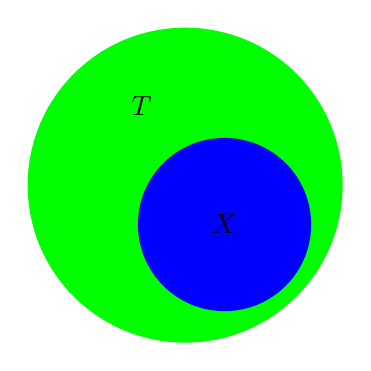
\begin{tikzpicture}
\draw [fill=green,draw=none] (-0.5,0.5) circle (2cm) node [color=black, left, xshift=-0.3cm, yshift=1cm] {$T$};
\draw [fill=blue,draw=none] (0,0) circle (1.1cm) node[color=black] {$X$};
\end{tikzpicture}
\end{center}

\section{Stochastic Programming}

\subsection{Motivation}

In this chapter we will explore optimization under uncertainty; in other words,
linear programming where some of our decision variables are stochastic.

We begin with a small example where a steel mill must plan a production schedule
to cater for future demand.

As production of the steel takes 3 months, the future market demand at $t=0$ is 
not known. However, the firm must allocate the right amount of resources for
mining and treating ore now.

\subsection{Feasibility Sets}\label{sec:spforms}

For the first stage:

\[
K_1 = \{ \bx \geq 0 : Ax = b \}
\]

Second stage \emph{elementary feasbility set}:

\[
K_2(\xi) = \{\bx : \mathscr{Q}(x,\xi) < \infty \} =  \{\bx : \exists \by \geq 0, \bW\by  = \bh - \bT\bx \}
\]

For continuous $\xi$ we define the \emph{possibility interpretation}:

\begin{alignat*}{2}
& K_2(\xi) = \{\bx : \mathscr{Q}(x) < \infty \} \\
& K_2^P(\xi) = \mathop{\cap}_{\xi \in \Xi} K_2(\xi) 
\end{alignat*}

$K_2 = K_2^P(\xi)$ holds when $\Xi$ is finite, as the following theorem states:

\begin{thm}\hfill\break
If $\Xi$ has finite second moments and $W$ is fixed, then $K_2 = K_2^p$
\end{thm}

\begin{proof}
For $K\subseteq K_2^p$, if $x \in K_2 \Rightarrow \mathscr{Q}(x) < \infty \Rightarrow 
\mathbb{E}_\xi\big[\mathcal{Q}(x,\xi)\big] < \infty \Rightarrow 
\underbrace{\mu (\mathcal{Q}(x,\xi)) = 2}_{\textrm{Probabilities sum to 1}}$.

We now have to show that $\{ \xi : \mathcal{Q}(x,\i)<\infty\}$ is a closed set.
\end{proof}

\begin{thm}\hfill\break
{\bf a)} For a given $\xi$, $K_2(\xi)$ is a convex polyhedron.\\
{\bf b)} When $\xi$ is a finite discrete random variable, $K_2$ is a convex polyhedron.
\end{thm}

\begin{proof}\hfill\break
{\bf a)} For some $x$ in the elementary feasbility set, that is,
\[
x \in K_2(\xi) = \big\{ x : \exists y \geq 0 : W y = h - Tx \big\}
\]

where the following is equivalent:

\[
h-Tx \in \text{pos}W = \big\{ t : \exists y \geq 0 : W y = t \big\}
\]

where pos$W$ is the positive cone of $W$. pos$W$ is a non-empty closed convex set, which
can be see since $0\in \text{pos}W$, \texttt{<insert closed/convex set proof>}, and it is
a cone since $\forall \lambda \in \mathbb{R}^{m_1}, t\in \text{pos}W \Rightarrow \lambda t \in
\text{pos}W$.\\

Due to the properties of pos$W$, we know that $\exists \{t : \sigma^\top t = \alpha\}$ such
that

\[
\sigma^\top (h-Tx) > \alpha
\]

and

\[
\text{pos}W \subseteq \{t : \sigma^\top t \leq \alpha\}
\]

Then, $0\in \text{pos}W \Rightarrow \alpha \geq 0$, and hence

\[
\sigma^\top (h-Tx) > \alpha \geq 0
\]

We prove by contradiction, i.e. if we can find $x$ such that $x\notin K_2(\xi)$ then
$h - Tx \notin \text{pos}W$. Then the separating hyperplane theorem tells us that we
can find a hyperplane $\big\{ t : \sigma^T t = \alpha \big\}$ such that

\[
h-Tx \in \big\{ t : \sigma^T t \geq \alpha \big\}
\]

and

\[
\text{pos}W \subseteq \big\{ t : \sigma^T t < \alpha \big\}
\]

However, because $\bm{0} \in \text{pos}W \Rightarrow \bm{0} \in \big\{ t : \sigma^T t < \alpha \big\}$
Therefore we must have that $\alpha > 0$.

Because $h-Tx$ is on the the other side of the cone we have $\sigma^T (h-Tx) \geq \alpha > 0$.


We now assume the opposite: $\exists t\in \text{pos}W : \sigma^T t\geq 0$. But
if $t\in \text{pos}W \Rightarrow \lambda t\in \text{pos}W \forall \lambda \in \mathcal{R}_n^+
\Rightarrow \lambda \sigma^T t \leq \alpha, \forall \lambda > 0$. This is a contradiction
because as $\lambda \rightarrow \infty, \lambda \sigma^T t < x$ cannot hold!
Therefore $\{ t: \sigma^T t = 0\}$ is a separating hyperplane!\\

Since there are be lots of separating hyperplanes $M = \{ \sigma : \forall t \in \text{pos}W :
\sigma^T t < 0\}$ this means that if $x\in K_2(\xi) \Leftrightarrow h-Tx \in \text{pos}W
\Leftrightarrow \sigma^T(h-Tx) < 0, \forall \sigma \in M$.

We arrive at the following conclusion: being in the elementary feasibility set means
being on the right side of all separating hyperplanes $\sigma \in M$.\\

$M$ is a non-empty convex cone: $\sigma^T (h-Tx) \leq 0, \forall \sigma \in M \Leftrightarrow
\sigma_i^T(h-Tx) < 0, i=1,..,|M|$.

Therefore, being in the elementary feasibility sets is the same as satisfying $|M|$ linear
inequalities, therefore $K_2$ is a polyhedron.
\end{proof}

\begin{proof}{\bf b)}
Let $\Xi = \{\xi_1, .., \xi_S\}$ (finite support) with $\prob{\xi(\omega)=\xi_s)} = p_s,\; s=1,..,S$.
$x\in K_2 \Leftrightarrow \mathcal{Q}(x) < \infty \Leftrightarrow \sum_{s=1}^S p_s
\mathcal{Q}(x,\xi_s) < \infty \Leftrightarrow \mathcal{Q}(x,\xi_s) < \infty, s=1,..,S
\Leftrightarrow x\in K_2(\xi_s), s=1,..,S = \cap_{s=1}^S K_2(\xi_s)$.
%The intersubsection of 
\end{proof}

Polyhedrons give rise to cutting-plane algorithms as we will see in subsection \ref{sec:lshape}.

The following theorem describes properties of the recourse function $\Q(x,\xi)$:

\begin{thm}\hfill\break
For a given $\xi$, $\Q(x,\xi)$ is\\
{\bf a)} piecewise linear convex in $(h,T)$.\\
{\bf b)} piecewise linear concave in $q$.\\
{\bf c)} piecewise linear convex in $x \forall x\in K_2$.
\end{thm}

\begin{proof}{\bf a)} and {\bf c)}\\

\end{proof}

\begin{proof}{\bf b)}
$\Q(x,\xi)$ = min $\{q^Ty : Wy = h-Tx, y\geq0 \}$
            = min $\{q^Ty_i : i=1,..,n\}$ where $y_i$ are the extreme points of $\{ y:  Wy = h-Tx, y\geq0 \}$ 
\end{proof}



\subsection{Formulations}

We will look at:

\begin{itemize}
\item First-order problems (use mean)
\item Second-order (scenarios)
\item Expected Value solution
\item EVPI
\item VSS
\end{itemize}

\subsubsection{Two-stage recourse problem}

This is the most basic type of stochastic program, namely where we only consider two stages
with fixed recourse (i.e. $\bm{W}$ is fixed).\\

\stone\\

Determine first-stage variable $\bx$.\\

\obs\\

$\xi(\omega)$\\

\sttwo\\

Make second-stage decisions based on the new information.\\

\form\\

This is an \emph{deterministic equivalent}:

\begin{alignat*}{2}
\textrm{min} & \quad \bm{c}^T \bx + \mathbb{E}_\xi \Big[\text{min } q(\omega)^Ty(\omega)\Big] \ & \ \\
\text{s.t.}  & \quad \bm{Ax} = \bm{b} & \ \\
             & \quad  \bm{T}(\omega)\bx + \bm{W}y(\omega) = h(\omega), & \ \\
             & \quad \quad x \in \mathcal{X} & \
\end{alignat*}

The first constraint represents the deicison we made in the first stage, while the
second constraint links the first and second stages.

\subsubsection{Multistage recourse problem}

\textbf{Implicit form}

\[
\text{min} \{ c^T x + \mathbb{E}_\xi \Q(x,\xi) : Ax=b, x\in X \}
\]

where $\xi$ is the random vector containgin the information we observe in the
second stage and

%\marginnote{The right-most expression is a probability-weighted sum!}
\[
\Q(x, \xi) = \text{min} \{ q^T y : Wy = h - Tx, y \geq 0 \}
           %= \sum_{s=1}^S p_s \Q^s(x)
\]

A more condensed implicit representation:

\[
\text{min} \{ c^T x + \mathscr{Q}(x) : Ax=b, x\in X \}
\]

where $\mathscr{Q}(x) = \mathbb{E}_\xi \Q(x,\xi)$.

This formulation is also called the \emph{deterministic equivalent}, since we
can compute the expectation in the first stage.

\textbf{Extensive form}

Assume that $\xi$ has a discrete distribution with finite support $\Xi = \{\xi_1, .., \xi_S\}$
such that

\[
\mathcal{P}\big[\xi(\omega) = \xi_s\big] = p_s,\quad \quad s=1..S
\]

\begin{alignat}{2}
\textrm{max} & \quad \bm{c}^T \bx + \mathbb{E}_{\xi_2}\Big[\text{min }c^2(\omega)^\top x^2(\omega) + \ldots + \mathbb{E}_{\xi_T}\big[
\text{min }c^T(\omega)^\top x^T(\omega) \big]\ldots\Big]& \ \\
\text{s.t.}  & \quad \bm{T}_1^s x_1^s = \bm{b}_1, \quad \quad s=1..S\ \\
             & \quad \bm{T}_{t-1}^s \bx_{t-1}^s + \bm{W}_t x_t^s = h_t^s, \quad \quad s=1..S\ \\
             & \quad \quad x_t^s = x_t^{s'}, \qquad \text{if } \big[ \xi_1^s, ..., \xi_t^s \big] = \big[ \xi_1^{s'}, ..., \xi_t^{s'} \big], t=2..T, s=1..S \ \label{eq:nonanti} \\
             & \quad \quad x_1^s \in \mathcal{X}_1, .. x_t^s \in \mathcal{X}_T & \ \\
\end{alignat}

This is a solvable linear program, but it is quite large due to the number of constraints.

\textbf{General Formulation}

Given the probability space $(\Omega, \mathcal{F}, \{ \mathcal{F}_{t} \}_{t=1}^T, \mathcal{P})$ 
with $\mathcal{F}_t \subseteq \mathcal{F}_{t+1}$ where $\mathcal{F}_1 = \emptyset$, 
$\mathcal{F}_T = \mathcal{F}$ we can formulate a multi-stage recourse problem as follows:

\begin{alignat}{2}
\textrm{max} & c_1 x_1 +  & \\
\text{s.t.}  & \quad \bm{T}_1^s x_1^s = \bm{b}_1, & \quad \quad s=1..S\ \\
             & \quad \quad x_1^s \in \mathcal{X}_1, .. x_t^s \in \mathcal{X}_T & \ \\
\end{alignat}

\textbf{Nodal formulation}

A nodal formulation use \emph{scenario trees}, as depicted in figure \ref{fig:stex}.

% Set the overall layout of the tree
\tikzstyle{level 1}=[level distance=3.5cm, sibling distance=3.5cm]
\tikzstyle{level 2}=[level distance=3.5cm, sibling distance=2cm]
\tikzstyle{circ} = [circle, minimum width=3pt,fill, inner sep=0pt]
\begin{figure}[h!]
\begin{center}
\begin{tikzpicture}[grow=right, sloped]
\node[circ] {}
    child {
        node[circ] {}        
            child {
                node[circ, label=right:
                    {$s_4$}] {}
                edge from parent
                %node[above] {$W$}
                %node[below]  {$\frac{4}{9}$}
            }
            child {
                node[circ, label=right:
                    {$s_3$}] {}
                edge from parent
                %node[above] {$B$}
                %node[below]  {$\frac{5}{9}$}
            }
            edge from parent 
            %node[above] {$W$}
            %node[below]  {$\frac{4}{7}$}
    }
    child {
        node[circ] {}
        child {
                node[circ, label=right:
                    {$s_2$}] {}
                edge from parent
                %node[above] {$B$}
                %node[below]  {$\frac{3}{9}$}
            }
            child {
                node[circ, label=right:
                    {$s_1$}] {}
                edge from parent
                %node[above] {$W$}
                %node[below]  {$\frac{6}{9}$}
            }
        edge from parent         
            %node[above] {$B$}
            %node[below]  {$\frac{3}{7}$}
    };
\end{tikzpicture}
\end{center}
\caption{An example of a scenario tree.}
\label{fig:stex}
\end{figure}

\begin{itemize}
\item $\mathcal{N}$ : nodes
\item $o$ : root
\item $\mathcal{N}_+(n)$ : successors of node $n$
\item $p^{n/n-}$ : transition probability
\item $p^n$ : probability of being in $n$, $\; p^n = p^{n-} p^{n/n-}, \quad n \in \mathcal{N} \setminus \{0\}$ 
\end{itemize}

Such a formulation obviates the need for non-anticipativity constraints since we always know the predecessor
node $n^-$.

W have $m|N|$ constraints and $n|N|$ variables.

\subsubsection{Chance Constrained Formulation}

Assuming we know the distribution of the underlying scenarios we may formulate the
probability in terms of quantiles. Consider the following example the UFL problem with
stochastic demand; i.e. $\xi = \{d_1, .., d_j\}$.

\begin{alignat*}{2}
\textrm{max} & \quad \bm{c}^T \bx + \sum_{j=1}^m \sum_{i=1}^n q_{ij} y_{ij}\ & \ \\
\text{s.t.}  & \quad\; y_{ij} \leq M x_j \ & \quad \quad j = 1..m, i = 1..n\ \\
             & \quad \prob{\sum_{j=1}^m y_{ij} \geq d_i(\omega)} \geq \alpha_i \ & \quad \quad i=1..n \\
             & \quad \quad x \in \mathcal{B}^1, y_{ij} \geq 0, \ & \quad \quad j = 1..m, i = 1..n
\end{alignat*}

\subsubsection{Elimination of Recourse Variables}

Assume $W = [I,-I]$, $q^T = ((q^+)^T, ((q^-)^T)$ and $y^T = ((y^+)^T, ((y^-)^T)$.\\

{\it First stage}:

\[
min \{ c^T x + \mathcal{Q}(x) : Ax=b, x\in X\}
\]

{\it Second stage} (we make the assumption that it is linear)

\[
\mathcal{Q}(x) = \mathbb{E}_{\xi}\big[ \mathcal{Q} x, \xi(\omega) \big]
\]
\[
\mathcal{Q}(x) = \text{min} \{\bq^+(\omega)\by^+ + \bq^-(\omega)\by^- : \by^+ - \by^- = \bm{h}(\omega) - \bm{T}(\omega)\bx, \by^+, \by^- \geq 0 \}
\]

Now, since nothing links the $\by$ variables we may decompose the minimization problem
above to a sum:

\[
= \sum_{i=1}^{n_2} \text{min} \{q_i^+(\omega)y_i^+ + q_i^-(\omega)y_i^- : y_i^+ - y_i^- = h_i(\omega) - \bm{T}_i(\omega)\bx, y_i^+, y_i^- \geq 0 \}
\]


Taking the example from before, the random recourse variables $y^+$ and $y^-$ are
complementary\footnote{Check definition from Trine's article!}, meaning that $y^+ y^- = 0$.i
We substitute the random recourse varibles:

\[
= \sum_{i=1}^{n_2} \{q_i^+(\omega)[h_i(\omega) - \bm{T}_i(w)x]^+ + q_i^-(\omega)[\bm{T}_i(w)x - h_i(w)]^+ : q_i^+(\omega) + q_i^-(\omega) \geq 0 \}
\]

\subsubsection{Second-stage Integer Variables}

Paper to \LaTeX is marked \# 1313

\subsubsection{Example: UFL}

The uncapacitated facility location problem is an example of a simple recourse problem.
The random vector $\xi$ is defined as follows:

%\[
%\bm{\xi} = (\bm{v, r, t_1, ..., t_m, d)}
%\]

where

\begin{itemize}
\item $\bm{v}:$ variable cost vector
\item $\bm{r}:$ price vector
\item $\bm{t}:$ transportation cost for each customer $i=1..m$
\item $\bm{d}:$ demand vector
\end{itemize}

\stone\\

Determine $x_j$, $y_{ij}$ (opening facilities and distribution).\\

\obs\\

$\bm{v_j(\omega), r_j(\omega), t_{ij}(\omega),d_j(\omega)}$\\

\sttwo\\

Based on the realization of $\xi$ we can now determine the shortages
and surplusses at each customer denoted by $w_i^+(\omega)$ and $w_i^-(\omega)$,
respectively.\\

\form

\begin{alignat*}{2}
\textrm{max}  & \quad  -\sum_{j=1}^m c_j x_j + \mathbb{E}_\xi \Big[\sum_{j=1}^{m} \sum_{i=1}^{n} (v_j(\omega) + t_{ij}(\omega))y_{ij})\Big] + \mathbb{E}_\xi \Big[\sum_{i=1}^n r_i(\omega)d_i(\omega)\Big]\ \\
 & \quad - \mathbb{E}_\xi \Big[\sum_{i=1}^n q_i^+ w_i^+(\omega) + q_i^- w_i^-(\omega)\Big]\ \\
\text{s.t.} & \quad \quad \sum_{j=1}^m y_{ij} + w_i^+(\omega) - w_i^-(\omega) = d_i(\omega),\ & i = 1..n\ \\
            & \quad \quad y_{ij} \leq M x_{ij}, & j=1..m, \; i = 1..n \ \\
            & \quad \quad x_j \in \mathcal{B}^1, y_{ij}, w_i^+, w_i^- \geq 0 & \
%\text{s.t.} & \quad \sum_{i=1}^m a_{ij} + e_j t_j \geq g_j &,\ & 1\leq j\leq n\\
\end{alignat*}

The recourse variables in in the programme above are $w_i^+$ and $w_i^-$. By observing that 

\[
w_i^+ = \mathbb{E}_\xi \Big[ d_i(\omega) + \sum_{j=1}^m y_{ij} \Big]^+
\]

and

\[
w_i^- = \mathbb{E}_\xi \Big[\sum_{j=1}^m y_{ij} - d_i(\omega) \Big]^+
\]

we may eliminate the recourse variables by substitution (also called \emph{simple recourse}):

\begin{alignat*}{2}
\textrm{max}  & \quad  -\sum_{j=1}^m c_j x_j + \mathbb{E}_\xi \Big[\sum_{j=1}^{m} \sum_{i=1}^{n} (v_j(\omega) + t_{ij}(\omega))y_{ij})\Big] + \mathbb{E}_\xi \Big[\sum_{i=1}^n r_i(\omega)d_i(\omega)\Big]\ \\
 & \quad - \Big[\sum_{i=1}^n q_i^+ \mathbb{E}_\xi \Big[ d_i(\omega) + \sum_{j=1}^m y_{ij} \Big]^+ + q_i^- \mathbb{E}_\xi \Big[\sum_{j=1}^m y_{ij} - d_i(\omega) \Big] \Big]\ \\
\text{s.t.} & \quad \quad \sum_{j=1}^m y_{ij} = d_i(\omega),\ & i = 1..n\ \\
            & \quad \quad y_{ij} \leq M x_{ij}, & j=1..m, \; i = 1..n \ \\
            & \quad \quad x_j \in \mathcal{B}^1, y_{ij}, w_i^+, w_i^- \geq 0 & \
\end{alignat*}

We say that the problem exhibits \emph{simple} recourse when we can eliminate
variables in this manner.

\subsection{Value of Stochastic Programming}

For a given stochastic programing problem, we have four different ways of solving
the problem:

\[
RP : \textrm{min  } \mathbb{E}_\xi{\big[z(x,\xi)\big]}, \; x \in K_1 \cap K_2(\xi)
\]

\[
WS : \mathbb{E}_\xi \big[\textrm{min }_x z(x, \xi) \big]
 %= \mathbb{E}{\big[\textrm{min  } z(\overline{x}(\overline{\xi}), \xi)\big]}
\]

\[
EV : \textrm{min  } z(x, (\overline{\xi})), \quad \mathbb{E}\big[\xi\big] = \overline{\xi}
\]

For the $EV$, we still have the recourse problem, we just do not care about the
stochasticity.

We also have the Expected Value of the $EV$:

\[
EEV : \mathbb{E}\big[ z(\overline{x}(\overline{\xi}), \xi) \big]
\]

The following proposition shows their relationship:

\begin{proposition}
$WS \leq RP \leq EEV$
\end{proposition}

\begin{proof}
We always have $z(\overline{x}(\xi), \xi) \leq z(x^*, \xi)$ regardless of $\xi$. Taking
the expectation on both sides shows the first inequality. 

For $RP\leq EEV$, it is clear that $\textrm{min  }_{x \in K_1 \cap K_2(\xi)} \mathbb{E}_\xi{\big[z(x,\xi)\big]}
\leq \mathbb{E}_\xi \big[z(\overline{x}(\overline{\xi}), \xi)\big]$.
If $\overline{x}(\overline{\xi})\notin K_2$, the recourse function takes on the value
$\infty$, so the inequality still holds.
\end{proof}

\begin{proposition}
If $q,\; W,\; T$ are fixed, then $EV \leq WS$.
\end{proposition}

\begin{proof}
Let $f(\xi) = \textrm{min}_{x\in K_1 \cap K_2(\xi)}$. $f$ is convex in $\xi$ because we
have already proved that $f$ is convex in its RHS.\\
By Jensen's inequality we have:

\[
\mathbb{E}_\xi \big[f(\xi)\big] \geq f(\mathbb{E}_\xi\big[\xi\big])
\Leftrightarrow WS \geq EV
\]

\end{proof}

We now define the \emph{expected value of perfect information} (EVPI) and \emph{value of
the stochastic program} (VSS) as the distances between the above formulations in terms
of objective value, so as to assess their utility.

\[
EVPI = RP - WS
\]

\[
VSS = EEV - RP
\]

We assume $EVPI, VSS \geq 0$.
Figure \ref{fig:valuesofsp} shows the relationship between these problems graphically.

\begin{figure}[h!]
\begin{center}
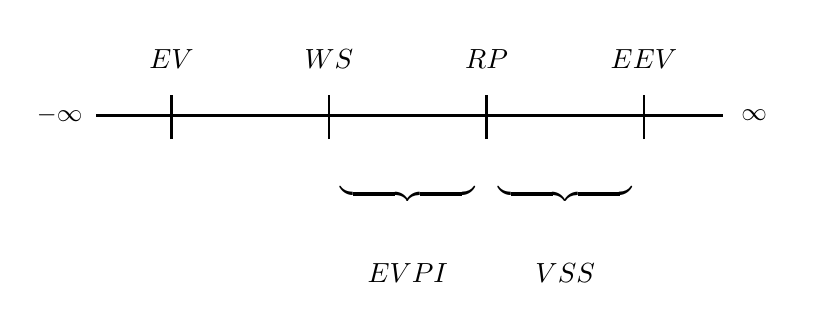
\begin{tikzpicture}[-,shorten >=1pt,auto,node distance=1.5cm,thick,minimum size=0.8cm,main node/.style={circle,draw=red,very thick}]
\tikzstyle{selected edge} = [draw,line width=6pt,-,blue!30]
\coordinate (origo) at (0,0);
\coordinate (EV) at (0,1);
\coordinate (WS) at (0,3);
\coordinate (RP) at (0,5);
\coordinate (EEV) at (0,7);

% Draw axes
\draw[-] (8,0) -- (origo) node[left] {\small $-\infty$};
\draw[-] (1,-0.3) -- (1,0.3) node[above] {$EV$};
\draw[-] (3,-0.3) -- (3,0.3) node[above] {$WS$};
\draw[-] (5,-0.3) -- (5,0.3) node[above] {$RP$};
\draw[-] (7,-0.3) -- (7,0.3) node[above] {$EEV$};
\node[] at (8.4,0) {\small $\infty$};

\node[] at (4,-1) {$\underbrace{\phantom{\hspace{1.7cm}}}$};
\node[] at (4,-2) {$EVPI$};

\node[] at (6,-1) {$\underbrace{\phantom{\hspace{1.7cm}}}$};
\node[] at (6,-2) {$VSS$};

\end{tikzpicture}
\caption{Relationship between $EV$, $WS$, $RP$ and $EEV$ for a minimization problem with fixed $q$, $W$ and $T$.}
\label{fig:valuesofsp}
\end{center}
\end{figure}

\subsubsection{Example}

Observe the following two-stage stochastic program\footnote{For ease of exposition I 
will use colours to keep track of what variables go where.} :

\[
\textrm{min } \{ 6x + \mathcal{Q}(x) : x\geq 0 \}
\]

where

\[
\mathcal{Q}(x) = \textrm{min } \{ 10y, y \geq x-\xi, y \geq \xi-x \}
\]

and $\textcolor{blue}{\xi_1} = \textcolor{blue}{\frac{1}{3}}$, $\textcolor{blue}{\xi_2} = 
\textcolor{blue}{\frac{2}{3}}$, $\textcolor{purple}{p_1} = \textcolor{purple}{\frac{1}{2}}$
and $\textcolor{purple}{p_2} = \textcolor{purple}{\frac{1}{2}}$.\\

\textbf{Computing $WS$}

For each $\xi$:

\[
\textrm{min } \{ 6x + 10|x-\textcolor{blue}{\frac{1}{3}}|: x\geq 0 \} = 2,\;\; 
\overline{x}(\textcolor{blue}{\frac{1}{3}}) = \frac{1}{3}
\]

\[
\textrm{min } \{ 6x + 10|x-\textcolor{blue}{\frac{2}{3}}|: x\geq 0 \} = 2,\;\; 
\overline{x}(\textcolor{blue}{\frac{2}{3}}) = \frac{2}{3}
\]

$WS = \textcolor{purple}{\frac{1}{2}}\cdot 2 + \textcolor{purple}{\frac{1}{2}}\cdot 4 = 3$

\textbf{Computing $EV$}

$\mathbb{E}\big[\xi\big]= \textcolor{purple}{\frac{1}{2}}\cdot \textcolor{blue}{\frac{1}{3}} 
+ \textcolor{purple}{\frac{1}{2}}\cdot \textcolor{blue}{\frac{2}{3}} = \textcolor{orange}{\frac{1}{2}}$

\[
\textrm{min } \{ 6x + 10|x-\textcolor{orange}{\frac{1}{2}}|: x\geq 0 \} = 3,\;\; 
\overline{x}(\textcolor{orange}{\frac{1}{2}}) = \textcolor{red}{\frac{1}{2}}
\]

\textbf{Computing $EEV$}

\begin{alignat*}{2}
EEV & = \textcolor{purple}{\frac{1}{2}}\big(6 \textcolor{orange}{\frac{1}{2}} + 10|\textcolor{orange}{\frac{1}{2}} - \textcolor{blue}{\frac{1}{3}}|) \\
& + \textcolor{purple}{\frac{1}{2}}\big(6 \textcolor{orange}{\frac{1}{2}} + 10|\textcolor{orange}{\frac{1}{2}} - \textcolor{blue}{\frac{2}{3}}|) \\
& = 4\frac{2}{3}
\end{alignat*}

\textbf{Computing $RP$}

\begin{alignat*}{2}
RP & = \textrm{min } \{ 6x + \textcolor{purple}{\frac{1}{2}}\big(10|\textcolor{red}{\frac{1}{2}} - \textcolor{blue}{\frac{1}{3}}|)
+ \textcolor{purple}{\frac{1}{2}}\big(10|\textcolor{red}{\frac{1}{2}} - \textcolor{blue}{\frac{2}{3}}|)\} \\
& = 3\frac{2}{3},\;\; x^* = \frac{1}{3}
\end{alignat*}

\subsection{Scenario Generation}

This subsections discusses different ways of generating data for input to our
stochastic programs. Also, it is often convenient for our input variables to
have certain statistical properties (moments).

\subsubsection{Moment Matching}

Moment matching is a way of generating these input data by solving a nonlinear
program that minimizes the square error of our realizations against the moments
we wish to match.

\begin{alignat*}{2}
\textrm{min}& \quad \quad \sum_{V_s} w_i \big[ f_i(\xi, p) - V_i \big]^2 \ \\
\text{s.t.} & \quad \quad \sum_{s=1}^S p_s = 1 & \ \\
            & \quad \quad p_s \geq 0, \; s=1..S & \
\end{alignat*}

where $w_i$ are weights e.g. a higher value of $w_i$ will cause an NLP solver to
minimize the error for the moment even more.\\

{\large\bf Pros \& Cons of Moment Matching:}
\begin{itemize}
\item[-] One large non-convex program is hard to solve
\item[-] How do we model dependencies between nodes?
\item[-] Might not produce the optimal solution
\item[-] Inconsistencies in probabilities due to datasets differing in size
\item[+] Independent of the size of the data set
\item[+] No knowlege of $\xi$ assumed
\item[+] Under/overspecification of $\xi$
\item[+] Weights = "faith"
\end{itemize}

If the number of moments and the numer of scenarios match, moment matching typically
performs well. If we were to increase the number of moments we wished to match, we 
would at some point \emph{overspecify} the distribution,. An example could be that that
we would not have enough variables to fully represent the covariance in the
distribution.\\

On the other hand, if we required more scenarios than moments, for instance
only matching the first moment for a larger number of scenarios, we could risk 
that every scenario except one that attains the mean value with probability one.

\subsubsection{Sampling Methods}

The solution to

\[
\hat{z} = \textrm{min}_{x \in \mathbb{X}} \frac{1}{S}\sum_{s=1}^S z(x,\xi_s)
\]

is called the \emph{sample average approximation}. If $\xi_1,..,\xi_S$ are i.i.d.,
then by the Law of Large Numbers:

\[
\hat{z} = \textrm{min}_{x\in \mathbb{X}} \frac{1}{S}\sum_{s=1}^S z(x,\xi_s) \rightarrow \mathbb{E}_\xi \big[z(x,\xi)\big]
\]

{\large\bf Pros \& Cons of Sampling:}
\begin{itemize}
\item[-] Many samples required, large SP, harder to solve ($S^N$ scenarios is $\xi \in \mathbb{R}^N$)
\end{itemize}

\subsubsection{Scenario Reduction}

Since the amount of nodes required for non-trivial problems increases exponentially
in the amount of stages, it is convenient to reduce this amount to make the problem
computationally tractable. As we will see, we may delete a subset of the initial set
of nodes $I = \{1, .., S\}$ in a methodical way. This subsection is dedicated to scenario
reduction which address the following question:\\

\begin{center}
Given $I = \{1, .., S\}$ of initial scenarios, which ones do we chose to delete?
\end{center}

In other words, we seek to find $J \subset I$.


\begin{alignat}{1}
P_d: d(I, q) = \text{min} \Big\{\sum_{i\in I} \sum_{j\notin J} c_{ij} \eta_{ij} : \eta_{ij} \geq 0, \;\sum_{j\notin J} \eta_{ij} = p_i, \;\sum_{i\in I} \eta_{ij} = q_j, i \in I, j \notin J \Big\}
\label{eq:distanceprimal}
\end{alignat}


If we fix the cardinality $k = |J|$, we solve the scenario reduction problem using the
following algorithm:\\

\begin{enumerate}
\item Compute distances between scenarios 
\item Chose scenarios to deleted based on distances (and previous choices)
\item Redistribute probabilities
\end{enumerate}


\begin{thm}\hfill\break
Given $J \subset I$, 

\[
D_j = \text{min  } \{ d(J, q) : \sum_{j \notin S} q_j = 1, q_j \geq 0,
j \notin J \} = \sum_{i\in J} p_i \textrm{min }_{k\notin J} c_{ik}
\]

where $S$ is the set of scenarios, and $I$ is the set of scenarios we keep, with
optimal solution:

\[
q_j^{*} = p_j + \sum_{i \in J \cap J_j} p_i, \quad j\notin J
\]

where $ J_j = \{ i \in I : c_{ij} = \text{min  }_{k \notin J} c_{ik} \}$.
\end{thm}

\begin{proof}
We find upper and lower bounds for $D_j$ and see that the values for $q_j$ coincide
for fixed $J$.\\

We first take the dual of $P_d$ (\ref{eq:distanceprimal}):

\[
d(J, q) = \text{max  } \{\sum_{i\in I} p_i u_i + \sum_{j\notin J} q_jv_j : u_i+v_j \leq c_{ij}, i\in I, j\notin J \}
%\overline{v}_j=0, \
\]

We try to construct a feasible solution:\\
Let $\overline{u}_i = \text{min  }_{k\notin J} c_{ik}, \overline{v}_j=0, i\in I, j\notin J$\\
Clearly, $\overline{u}_i \leq c_{ij}$!
So a feasible solution is:

\[
\overline{u}_i  = \text{min  }_{k\notin J} c_{ik}
\]

\[
\overline{v}_j = 0
\]

If we insert this feasible solution:

\[
d(J,q) \geq \sum_{i\in I} p_i \text{min}_{k\in J} c_{ik} = \sum_{i\in J} p_i \text{min}_{k\in J} c_{ik}
\]

The last equality holds because the distance from the set $I$ to itself is zero. This holds for all $q$,
therefore also the $q$ that minimizes the distance i.e. the optimal value to the reduction problem has
the same lower bound:\\

\[
D_j \geq \sum_{i\in J} p_i \text{min}_{k\notin J} c_{ik}
\]

We now construct a feasible \emph{primal} solution for 

\begin{center}
$\eta_{ij} =
\begin{cases}
p_i & i\in J\cap J_j \;\text{ or }\; i=j, i\in I, j\notin J\\
  0 & 
\end{cases}$
\end{center}

and

\[
q_j = p_j + \sum_{i\in J \cap J_j} p_i,\quad j\notin J
\]

We must now show that this solution satisfies the following constraints:\\

\begin{enumerate}
\item $\overline{\eta}_{ij} \geq 0, i \in I, j\notin J$
\item $\sum_{j\notin J} \overline{\eta}_{ij} =
\begin{cases}
\overline{\eta}_{ik} & i\in J\cap J_k \;\text{ for some  }\; k\notin J\\
\overline{\eta}_{ii} & i\notin J
\end{cases}$
\item $\sum_{i\in I} \eta_{ij} = q_j$
\end{enumerate}

The first is trivially satisfied, and both piecewise constraints equate to $p_i$ by 
defition.
For the third we observe the following:\\

\[
\sum_{i\in I} \eta_{ij} = p_j + \sum_{i\in J\cap J_j} p_j = \overline{q}_j
\]

This is \emph{exactly} the definition, and is therefore a feasible solution. Hence,
we have an upper bound:

\begin{alignat*}{2}
d(J, \overline{q}) \leq \sum_{i\in I} \sum_{j\notin J} c_{ij} \overline{\eta}_{ij}
= \underbrace{\sum_{i \notin J}\sum_{j\notin J} c_{ij} \overline{\eta}_{ij}}_{\text{Keep}}
+ \underbrace{\sum_{i \in J}\sum_{j\notin J} c_{ij} \overline{\eta}_{ij}}_{\text{Goes away}} & \\
= \underbrace{\sum_{i\notin J} c_{ij} \overline{\eta}_{ij}}_{\text{distance from $I$ to $I$ = 0}}
+ \underbrace{\sum_{j\in J} p_i \text{min}_{k\notin J} c_{ik}}_{\text{Take the closest}}
= \sum_{j\in J} p_i \text{min}_{k\notin J} c_{ik}
\end{alignat*}

Now we just need to check if $\overline{q}_j \geq 0$ (given) sum to one:

\begin{alignat*}{2}
\sum_{j\notin J} q_j = \sum_{j\notin J} p_j + &\sum_{j\notin J} \sum_{i\in J\cap J_j}p_i\\
= \sum_{j\notin J} p_j + \underbrace{\sum_{i\in J} p_i}_{\text{=0}} & \\
= \underbrace{\sum_{j\notin J} p_j = 1}_{\text{From the definition}} &
\end{alignat*}

Thus we have proved that

\[
D_j \leq d(J,\overline{q}) \leq \sum_{i \in J} p_i\; \text{min}_{k\notin J} c_{ik}
\]

and we have a lower bound.
\end{proof}

So far, we have seen how to \_\_\_\_\_\_\_\_. We now go through how to select the
set $J\subset I$!

Given $D_j \forall J\subset I$, the reduction problem looks as follows:

\begin{equation}\label{eq:redprob}
D=\text{min} \big\{ \sum_{i\in J} p_i \text{min }_{k\notin J} c_{ik} : J\subseteq I, \left\vert{J}\right\vert = k\big\}
\end{equation}

In the following, let $J=\{l_1, .., l_k\}$ so the reduction problem is:

\begin{equation}
D=\text{min} \big\{ \sum_{i\in J} p_i \text{min }_{l\neq k} c_{ik} : l\in I \big\}
\end{equation}

As we saw, if we have an optimal solution $l^*$ we can easily redistribute the probabilites.

\begin{thm}
$\sum_{i=1}^k p_{l_i} \text{min}_{k\neq l_i} c_{ik} \leq D_k,\; i=1,..,k$
is a lower bound
\end{thm}

\begin{proof}
Let $J= \{j_1, .., j_j\}$, $|J| = k$, by theorem (link above):

\begin{alignat*}{2}
D_j = \sum_{i\in J} p_i \text{min}_{k\notin J} c_{ik} & = \sum_{i=1}^k p_i \text{min}_{k\in \{j_1, .., j_k\}} c_{ik}\\
& = \underbrace{\sum_{i=1}^k p_{j_i} \text{min}_{k \neq j_i} c_{j_i k}}_{\text{larger feasible region}} \\
& = \underbrace{\sum_{i=1}^k p_{l_i} \text{min}_{k \neq l_i} c_{l_i k}}_{\text{independent of } J}
\end{alignat*}

So it is a lower bound for \emph{any} $J$ (= $D_j$) , even the one that minimizes (= $D$)!
Hence

\[
D \geq \sum_{i=1}^k p_{l_i} \text{min}_{k\neq l_i} c_{l_i k}
\]
\end{proof}

So if for $i=1,..,k$, $\text{min}_{k\neq l_i} c_{l_i k}$ has an optimal solution $J=I\setminus \{l_1,..,l_k\}$,
then 

\[
D_j \geq \sum_{i=1}^k p_{l_i} \text{min }_{k\neq l_i} c_{l_i k}
= \sum_{i=1}^k p_{l_i} \text{min}_{k\in\{l_i,..,l_k\}} c_{l_i k} = D
\]

We now present an algorithm for the reduction problem:

\textsc{Backward Reduction Algorithm}

\begin{enumerate}
\item Initialize: $v=1$, $\mathcal{P}(v) = \mathcal{P}$, $I^{(v)} = I$.
\item Choose $J$ by selecting one element at a time:
  \begin{itemize}
  \item For $i=1,..,k^{(v)}$, solve
        \[
           \text{min}_{l \in I\setminus \{l_1,..,l_{i-1}\}} \text{min}_{k\neq l} c_{l_i k}
        \]
        and let $l_i$ be an optimal solution. If this solution is
  \item If the
  \end{itemize}
\item Redistribution. Let $J = \{l_1, ..,l_k\}$, $q_j = p_j^{v} + \sum_{i\in J\cap J_j} p_i^{v}$,
      where $j\notin J$, $J_j^{(v)} = \text{min} \{i\in I^{(v)} : c_{ij} = \text{min}_{k\neq j} c_{ik}\}$.
      If $K^{(v)} = K$ (???) terminate. If $K^{(v)} < K$, let $\mathcal{P}^{(v+1)} = Q$, $I^{(v+1)}=I^{(v)}\setminus J$,
      $k^{(v+1)} = K-something$ (???) and $v:= v+1$. Go to step 2.
\end{enumerate}


\subsection{Solution Methods for Stochastic Problems}\label{sec:lshape}

\begin{itemize}
\item Primal decomposition: stage relaxation
\item Dual decomposition: scenario relaxation
\end{itemize}

\subsubsection{Two-stage Problems}

Unless our problem exhibits complete recourse, we would like to select $x$ such
that all second-stage problems are feasible. As we saw in subsection \ref{sec:spforms},
if $\Xi$ has finite support, we have a finite number of linear constraints describing
our elementary feasbility set $K_2$. In this subsection we will see that we do not
always have to include all of these constraints in our problem, namely through a
method called $\mathcal{L}$-shaped decomposition.\\

We observe the implicit formulation for a two-stage problem:

\begin{alignat*}{2}
\textrm{min}  \quad & c^Tx +\Q(x) \ \\
\textrm{s.t.} \quad & x\in K_1 \cap K_2 & \
\end{alignat*}

which is equivalent to

\begin{alignat}{2}
\textrm{min}  \quad & c^Tx +\theta \ \\
\textrm{s.t.} \quad & x\in K_1 \cap K_2 \ \label{eq:spsol1}\\
                    & \theta \geq  \Q(x) \label{eq:spsol2} \
\end{alignat}

Recall that if our problem exhibits block structure, then for fixed $x$,
the problem decomposes into one subproblem per scenario.\marginnote{Draw this!}

The basic idea behind this solution method is to relax \ref{eq:spsol1}
and \ref{eq:spsol2} and introduce \emph{feasibility} and \emph{optimality}
cuts as necessary and end up with the \emph{Master} problem:

\begin{alignat}{3}
\textrm{min}  \quad & c^Tx +\theta & \ \\
\textrm{s.t.} \quad & x\in K_1  & \\
                    & D_l x           & \geq d_l, \quad l = 1,..,r \label{eq:spsolfc} \ \\
                    & E_l x  + \theta & \geq e_l, \quad l = 1,..,h \label{eq:spsoloc} \
\end{alignat}

where \ref{eq:spsolfc} are the feasibility cuts and \ref{eq:spsoloc} are 
optimality cuts. We now go through the steps of the L-shaped algorithm:\\

\textsc{L-shaped Algorithm}
\begin{itemize}
\item Feasibility check ($x^v \stackrel{?}{\in} K_2$):\\

We solve a slightly modified recourse problem per scenario:\\
\[
\Q'(x^v, \xi_s) = \textrm{min} \big\{ e^T v^+ + e^T v^- : Wy + Iv^+ - Iv^- = h_s - T_s x, y \geq 0 \big\}
\]
However, we would rather solve the dual of this:
\[
\Q_D'(x^v, \xi_s) = \textrm{max} \big\{ \sigma^T (h_s - T_s x) : \sigma^T W \leq 0, \pm \sigma^T \leq e^T \big\}
\]
since the constraints in the dual hold for any choice of $x$.

If indeed $x^v \in K_2(\xi_s)$ strong duality holds and

\[
\Q'(x^v, \xi_s) = \Q_D'(x^v, \xi_s)
\]

If $x^v \notin K_2(\xi_s)$ then:

\[
\Q'(x^v, \xi_s) > 0, \Q_D'(x^v, \xi_s) > 0, \sigma^T(h_s- T_s x) > 0
\]

But then $\sigma^T(h_s- T_s x) \leq 0$ cuts off $x^v$! This is 
exactly what we want, so we introduce the following constraint
in the Master problem (incrementing $r$ by one):

\[
D_{r} x \geq d_{r}
\]

where $D_{r} := (\sigma^v)^T T_s$ and $d_{r} := (\sigma^v)^T h_s$.

\item Optimality check ($\theta \stackrel{?}{\geq} \Q(x^v)$):\\

At this point, we know that $x^v$ is a feasible solution to

\[
\Q(x^v, \xi_s) = \textrm{min} \big\{ q_s^T y_s: Wy = h_s - T_s x^v, y \geq 0 \big\}
\]

However, the dual:

\[
\Q_D(x^v, \xi_s) = \textrm{max} \big\{ \pi^T (h_s - T_s x^v) : \pi^T W \leq q_s^T \big\}
\]

could be infeasible due to unbounded primal!\footnote{We assume $\Q(x^v, \xi_s)$
has a finite optimal solution so strong duality holds.}
We start by assuming $\theta < \Q(x^v)$. Then, by the same argument as for
feasibility cuts, we can introduce a constraint to cut off $x^v$:

\[
\theta < \Q(x^v) = \sum_{s=1}^S p_s \Q(x^v, \xi^s)= \sum_{s=1}^S p_s (\pi_s^v)^T(h_s - T_s x^v)
\]

hence

\[
\theta \geq \sum_{s=1}^S p_s (\pi_s^v)^T(h_s - T_s x^v)
\]

cuts off $x^v$, and is a valid for all $x$ since the $x^v$ does not appear in the
constraints in the dual. The actual constraint to introduce is then (incrementing $h$):

\[
E_{h} x + \theta \geq e_{h}
\]

where $E_{h} := \sum_{s=1}^S p_s (\pi_s^v)^T T_s$ and $e_h := \sum_{s=1}^S p_s (\pi_s^v)^T h_s$.

If $\theta \geq e_h - E_h x^v$ we can stop the algorithm since $x^v$ is optimal,

\end{itemize}

We now prove that the L-shaped algorithm converges.

\begin{thm}
Assuming $\Xi$ has finite support and a finite optimal solution the L-shaped algorithm
converves to an optimal solution in a finite number of iterations.
\end{thm}

\begin{proof}
$\Q(x^v, \xi_s)$ has only a finite number of bases, therefore a finite number of cuts
can be added. This means that $\exists v : v^v \in K_2, \theta^v \geq Q(x^v)$, hence
the algorithm terminates in a finite number of iterations.
Then:

\begin{alignat*}{2}
z^* & = \textrm{min} \big\{ c^T x + \Q(x) : x \in K_1 \cap K_2 \big\} \\
    & = \textrm{min} \big\{ c^T x + \theta : x \in K_1 \cap K_2, \theta \geq \Q(x) \big\} \\
    & \geq \textrm{min} \big\{ c^T x + \theta : x \in K_1, D_l x \geq d_l, l=1,..,s , E_l x + \theta \geq e_l, l=1,..,r \big\}
\end{alignat*}

\begin{alignat*}{2}
z^* & = \textrm{min} \big\{ c^T x + \Q(x) : x \in K_1 \cap K_2 \big\} \\
    & \leq c^Tx^v + \mathcal{Q}(x^v)
\end{alignat*}

we must have equality throughout, so $x^v$ is an optimal solution.
\end{proof}

The cuts we introduce might not include \emph{all} of the original ones, thus
we have a lower bound due to a larger feasible region.\\

\textsc{Multicut L-shaped Algorithm}\\

The problem:

\begin{alignat*}{2}
\textrm{min}  \quad & c^Tx + \sum_{s=1}^S p_s \Q(x,\xi_s) \\
\textrm{s.t.} \quad & x\in K_1 \cap K_2 & \\
                    & \theta_s \geq \Q(x) &
\end{alignat*}

is equivalent to:

\begin{alignat*}{2}
\textrm{min}  \quad & c^Tx + \sum_{s=1}^S p_s \theta \ \\
\textrm{s.t.} \quad & x\in K_1 \cap K_2 & \\
                    & \theta_s \geq p_s \Q(x, \xi_s), \quad s=1,..,S &
\end{alignat*}

Assume $\theta_s^v < p_s \Q(x^v, \xi_s)$. We do the same as before:

\[
\theta_s^v < p_s \Q(x^v, \xi_s) = p_s (\pi_s^v)^T
\]

Hence,

\[
\theta_s^v \geq p_s (\pi_s^v)^T(h_s - T_s x) 
\]

cuts off the solution $(x^v, \theta_1^v, .., \theta_s^v)$. We perform
feasbility check:

\textbf{Disaggregated vs. Aggregated}

\begin{itemize}
\item[-] More cuts, harder to solve the master problem due to bigger bases matrix
\item[+] Due to more cuts, we have more information about the recourse function, perhaps solve the master fewer times
\item[+] Cherry-pick some of the redundant constraints in the multicut version
\end{itemize}

\subsubsection{Two-stage Problems with Integral First Stage}

The problem is formulated as:

\[
\textrm{min } \{ c^Tx + \Q(x) : Ax=b, x\in \bX \}
\]

We note that the recourse function $\Q$ is still piecewise linear convex. If
$\xi$ has finite support, $K_2$ is a convex polyhedron (nothing has changed
in the second stage).
However, if $x\in \mathcal{Z}_+^{n_1}, y\in \mathcal{Z}_+^{n_2}$, $K_2$ and
$\Q$ are in general non-convex.\\

We present a solution method for this problem:

\begin{alignat}{2}
\textrm{min}  \quad & c^Tx + \theta \\
\textrm{s.t.} \quad & Ax=b & \\
                    & x\in K_2 & \label{eq:spi1} \\
                    & \theta_s \geq \Q(x) & \label{eq:spi2} \\
                    & x\in \mathcal{Z}_+^{n_1} \label{eq:spi3} &
\end{alignat}

As before, we we relax all difficult equations. Equation \ref{eq:spi1} and 
\ref{eq:spi2} and reintroduce them through feasibility and optimality cuts,
respectively. Equation \ref{eq:spi3} is handled through branch and bound algorithms.
%as seen in subsection \ref{sec:bnb}.\\
We end up with the master problem (where $x$ is only required to
non-negative):

\begin{alignat}{3}
\textrm{min}  \quad & c^Tx +\theta & \label{eq:spimaster1} \\
\textrm{s.t.} \quad & x\in K_1  & \label{eq:spimaster2} \\
                    & D_l x           & \geq d_l, \quad l = 1,..,r \\
                    & E_l x  + \theta & \geq e_l, \quad l = 1,..,h \\
                    & x \geq 0 \label{eq:spimaster3} 
\end{alignat}

\textsc{Branch and Cut for Stochastic Integer Programs}

\begin{itemize}
\item Set incumbent $\overline{z} = \infty$.
\item Root node: Solve initial master problem (equations \ref{eq:spimaster1}, 
\ref{eq:spimaster2}, \ref{eq:spimaster3})
\item Feasbility Check: $x^v \in K_2$, add feasbility cut as before.
  \begin{itemize}
     \item Prune by Bound: $c^Tx^v + \theta \geq \overline{z}$, fathom current node
     \item Check Integrality: $x^v \stackrel{?}{\in} K_2$, branch on fractional $x$.
\end{itemize}
\item Optimality Check: $\theta \stackrel{?}{\geq} \Q(x^v)$, otherwise add optimality
cut and solve the current problem in this node. If indeed $\theta \geq \Q(x^v)$,
we have a feasible solution and we may prune the node by optimality.
\end{itemize}

\begin{proposition}
The optimality cuts from the linear programming relaxation of the second stage are
still valid.
\end{proposition}

\begin{proof}\hfill\break
Let $c(x,\xi(\omega)) = \textrm{min }\{q(\omega)^\top y : Wy = h(\omega)-T(\omega)x, y\geq 0 \}$
and $c(x) = \mathbb{E}_\xi \big[ c(x,\xi(\omega)) \big]$. If $\theta \geq \Q(x) = \mathbb{E}_\xi
\big[ c(x,\xi(\omega)) \big]$ (convex, piecewise linear for finite $\Xi$).
\end{proof}

Problem: We cannot guarantee convergence of the algorithm!

\subsubsection{Two-stage Problems with Binary First Stage}

\begin{proposition}
Let $x^v$ be a feasible first stage solution. Let $S=\{ i: x_i^v = \}$ and
$q_s = \mathscr{Q}(x^v)$. Then,

\[
\theta \geq (q_s - L) \big(\sum_{i\in S}x_i - \sum_{i\notin S}x_i\big) -(q_s-L)(|S|-1)+L
\]

is a valid inequality.
\end{proposition}

\begin{proof}
Let $\delta(x,s) = \sum_{i\in S}x_i - \sum_{i\notin S} x_i$. Note that $\delta(x,s) \leq |S|$.
If $\delta(x,s) = |S|$ : $(q_s -L)\delta(x,S) - (q_s -L)(|S|-1)+L = q_s = \mathscr{Q}(x)\leq 
\theta$ so the cut is valid.\\
If $\delta(x,s) \leq |S|-1$ : $(q_s -L)\delta(x,S) - (q_s -L)(|S|-1)+L \leq L \leq \mathscr{Q}(x)
\leq \theta$.
So we add the cut $\theta \geq \mathscr{Q}(x) \Leftrightarrow \theta \geq (q_{s_l} -L)\delta(x,s) - (q_{s_l}-L)(|S_l|-1)+L \leq L \leq \mathscr{Q}(x)$ where $L -\leq 2^n$.

\end{proof}

We end up with one cut per feasible solution, resulting in potentially $2^n$ cuts and makes
it hard to solve.

\textbf{Improved Optimality Cuts for Binary First Stage}

We define an \emph{s-neighbour}:

\[
N(s,S) = \{ x\in \mathbb{B}^{n_1} : Ax=b, \delta(x,s) = |S|-s \}
\]

which is basically how many "bit-flips" required for a binary vector to be equivalent to
another.

\begin{proposition}
Let $x^v$ be a feasible first-stage solution. Let $S=\{i : x_i^v = 1\}$, $q_s = \mathscr{Q}(x^v)$,
$1 \leq t \leq |S|$ and $a = \textrm{max } \big\{\textrm{max }_{1\leq s\leq t} \{ (q_s -\lambda(s,S))/|S|\},
(q_s - L)/(t+1)\big\}$. Then,

\[
\theta \geq a(\sum_{i\in S} x_i - \sum_{i\notin S} x_i) + q_s + a|S|
\]

is valid and better for \emph{s-neighbours}.
\end{proposition}

\begin{proof}
We prove the theorem for $s=0$, $s\leq t$ and $s\geq t+1$. In all cases, let $x=x^v$:\\
$s=0$:

\[
\theta \geq a\delta(x,S) + q_s - a|S| = q_s = \mathscr{Q}(x) \leq \theta
\]

$s\leq t$:

\begin{alignat*}{2}
a\delta(x,S) + q_s - a|S| & =  a(|S|-s) + q_s - a|S|\\
& = q_s - a\cdot s\\
& \leq q_s - (q_s -\lambda(s,S))\cdot \frac{s}{S}\\
& = \lambda(s,S)\\
& \leq \mathscr{Q}(x)\\
& \leq \theta
\end{alignat*}

$s\geq t+1$:

\begin{alignat*}{2}
a\delta(x,S) + q_s - a|S|\\
& = q_s - a\cdot s \\
& \leq q_s - (q_s - L)\frac{s}{t+1} \\
& \leq L \\
& \leq \mathscr{Q}(x)\\
& \leq \theta
\end{alignat*}
\end{proof}

\subsubsection{Dual Decomposition}

The L-shaped method uses \emph{primal} decomposition i.e. decomposition w.r.t. stages.
We now present a way of solving stochastic programs by decomposing w.r.t scenarios,
meaning we relax non-anticipativity constraints in the explicit formulation (see
equation \_\_\_\_ for a reminder).\\

The problem size for the original problem is:\\
\marginnote{Move this to formulations!}

\hspace{2cm} \textbf{\# variables} $ = n_1 + n_2S$\\

\hspace{2cm}\textbf{\# constraints} $ = m_1 + m_2S$\\

We proceed by Lagrangian relaxation of the non-anticipativity constraints.
Assume $x_1 = ...= x_S$ can be expressed as a set of linear constraints in one of the
two following ways:

\begin{enumerate}
\item $\sum_{s=1}^S H_sx_s = 0$, where $H_s$ is a $\mathbb{R}^{l\times n_1}$ matrix.
      \[ H = \left( \begin{array}{rrrr}
      I & -I &    & \\
        &  I & -I & \\
        &    &  I & -I \end{array} \right)\]
\item $x_1 = x_j,\; j\in \{1,..,S\}$ (the j\textsuperscript{th} column is just ones in $H_s$, $s=1,..,S$)
\end{enumerate}

Let $J_s = \{ (x,y) : Ax=b, T_s x + Wy_s = h_s, x \in \mathbb{X}, y\in \mathbb{Y} \}$, that is the set of
feasible first and second-stage solutions per scenario.

We have the primal:

\begin{equation}\label{eq:lgprimal}
P: z = \textrm{min }\{ \sum_{s=1}^S p_s (c^\top x_s + q_s^\top y_s) : (x_s, y_s) \in J_s, s=1,..,S, 
\underbrace{\sum_{s=1}^S H_sx_s = 0}_{\textrm{Relax!}}\}
\end{equation}

\begin{equation*}
J_s = K_1 \cap K_2(\xi_s)
\end{equation*}

and the Lagrangian dual which decomposes nicely:

\begin{alignat*}{2}
D(\lambda) & = \textrm{min }\{ \sum_{s=1}^S p_s (c^\top x_s + q_s^\top y_s) + \lambda\sum_{s=1}^S H_sx_s : (x_s, y_s) \in J_s, s=1,..,S,\} \\
& = \sum_{s=1}^S \{ \textrm{min } p_s (c^\top x_s + q_s^\top y_s) + \lambda H_sx_s : (x_s, y_s) \in J_s\}\\
& = \sum_{s=1}^S D_s(\lambda)
\end{alignat*}

where each $D_s(\lambda)$ has the following problem sizes:\\

\hspace{2cm} \textbf{\# variables} $ = n_1 + n_2$\\

\hspace{2cm}\textbf{\# constraints} $ = m_1 + m_2$\\

The idea is to solve the Lagrangian dual:

\[
z_{LD} = \textrm{max } \{D(\lambda) : \lambda \in \mathbb{R}^l\}
\]

\begin{proposition}\hfill\break
{\bf i)}  $z_{LD} \leq z$\\
{\bf ii)} If $\exists \overline{\lambda}$ such that the optimal solutions $(\overline{x}_s,\overline{y}_s)$
to $D_s(\overline{\lambda})$, $s=1,..,S$ satisfies the non-anticipativity constraints, then $z_{LD} = z$ and
the solution is optimal to both the primal and dual problem.
\end{proposition}

\begin{proof}
{\bf i)} Let $\lambda \in \mathbb{R}^l$ and let $(\overline{x}_s,\overline{y}_s)$, $s=1,..,S$, be optimal
solutions to \ref{eq:lgprimal}. Then we obtain an upper bound 

\[
D(\lambda)\leq p_s(c^\top x_s + q_s^\top y_s)
\]

\[
\sum_{s=1}^S D(\lambda) \leq \sum_{s=1}^S p_s(c^\top x_s + q_s^\top y_s) \Leftrightarrow z_{LD} \leq z
\]

{\bf ii)}

\begin{alignat*}{2}
D(\overline{\lambda}) &= \sum_{s=1}^S D(\lambda) \leq \sum_{s=1}^S p_s(c^\top x_s + q_s^\top y_s)
  + \lambda\sum_{s=1}^S H_s\overline{x}_s\\
& = \sum_{s=1}^S p_s(c^\top x_s + q_s^\top y_s)
\end{alignat*}

assuming $(\overline{x}_1 = .. = \overline{x}_S)$. Therefore we have a feasible solution:

\[
\sum_{s=1}^S p_s(c^\top x_s + q_s^\top y_s) \geq z
\]

\[
z_{LD} = \textrm{max } \{ D(\lambda) : \lambda \in \mathbb{R}^l \} \geq z
\]
\end{proof}

\begin{proposition}\hfill\break
$z_{LD} = \textrm{min }\{ \sum_{s=1}^S p_s (c^\top x_s + q_s^\top y_s) : (x_s, y_s) \in \textrm{conv}(J_s), s=1,..,S, \sum_{s=1}^S H_sx_s = 0\}$
Something about the LG relaxation is at least as good as the LP relaxation.

We define $J_s^{LP}$ as the feasible region for the LP relaxation of each scenario:

\[
J_s^{LP} = \{ (x,y) : Ax=b, T_s x + Wy = h_s, x\geq 0, y\geq0 \}
\]

and so 

\[
J_s \subseteq \textrm{conv}(J_s) \subseteq J_s^{LP}
\]

and the ranking of the objective function values:

\[
z\geq z_{LD} \geq z_{LP}
\]
\end{proposition}

\begin{proof}
Assume $J_s = \{ (x_{is}, y_{is}) : i=1,..,T_s \}$. Then,

\begin{alignat*}{2}
z_{LD} & = \textrm{max } \{ D(\lambda) : \lambda \in \R^l \} \\
       & = \textrm{max } \{ \sum_{s=1}^S D_s(\lambda) : \lambda \in \R^l \} \\
       & = \textrm{max } \{ \sum_{s=1}^S \textrm{min }\{p_s(c^\top x_s + q_s^\top y_s) + \lambda H_s x_s : (x_s, y_s) \in J_s\} : \lambda \in \R^l \} \\
       & = \textrm{max } \{ \sum_{s=1}^S \textrm{min }\{p_s(c^\top x_{is} + q_s^\top y_{is}) + \lambda H_s x_{is} : i=1,..,T_s\} : \lambda \in \R^l \} \\
       & = \textrm{max } \{ \sum_{s=1}^S \eta_s : \eta_s \leq p_s(c^\top x_{is} + q_s^\top y_{is}) + \lambda H_s x_{is}, \lambda \in \R^l, i=1,..T_s, s=1,..,S \} 
\end{alignat*}

We take the dual of the last equation:

\begin{alignat*}{2}
\textrm{min } \big\{&\sum_{s=1}^S \sum_{i=1}^{T_s} \mu_{is} p_s(c^\top x_{is}+q_s^\top y_{is}) : \sum_{i=1}^{T_s} \mu_{is}=1,
  s=1,..,S,\\
& \sum_{s=1}^S \sum_{i=1}^{T_s} H_s x_{si} \mu_{is} = 0, \mu_{is}\geq 0, i=1,..,T_s, s=1,..,S \big\} \\
=\textrm{min } \big\{&\sum_{s=1}^S \sum_{i=1}^{T_s} \mu_{is} p_s(c^\top \Big(\sum_{i=1}^{T_s} \mu_{is}x_{is}\Big) + q_s^\top \Big(\sum_{i=1}^{T_s} \mu_{is}y_{is}\Big)) : \sum_{i=1}^{T_s} \mu_{is}=1, \\
& s=1,..,S, \sum_{s=1}^S \sum_{i=1}^{T_s} H_s \Big(\sum_{i=1}^{T_s} \mu_{is} x_{is}\Big) \mu_{is} = 0, \mu_{is}\geq 0, i=1,..,T_s, s=1,..,S \big\} \\
= \textrm{min }\{&\sum_{s=1}^S p_s (c^\top x_s + q_s^\top y_s) + \lambda\sum_{s=1}^S H_sx_s=0 : (x_s, y_s) \in \textrm{conv}J_s, s=1,..,S\} \\
\end{alignat*}

The last equality holds because $\sum_{i=1}^{T_s} \mu_{is} x_{is} = 1$ is a convex combination.
\end{proof}

For multistage programs, the dimension of $\lambda$ becomes very large as we relax the non-anticipativity constraints, making it harder to solve by subgradient algorithms.

\subsection{Risk Management}

Whenever we consider a problem with stochastic variables we have a notion of \textit{risk}\footnote{Assuming that hedging is not
possible}. In layman's terms, risk is the loss (usually measured in monitary terms) associated with unfavourable realisations of
$\xi$, where $\xi$ is the random variable affecting our outcome.\\

\subsubsection{Risk Measure 1: Value At Risk}

\emph{V@R is the probability of a decision $x$ resulting in losses below a given level $\alpha$}.

%loss intrinsic in a decision $x$ and probability $\beta$. Note that we speak in deterministic terms since we have
%indicated the desired probability. It can be thought of as an inverse cumulative distribution function of the losses for a
%given $x$.

Mathematically, it is defined as:

\[
\Psi(x,\alpha) = \int_{f(x,y) \leq \alpha} p(y) d(y)
\]

Next, we define $\alpha_\beta (x)$ ($\beta$-V@R) as the minimal losses incurred for a decision $x$ and probability $\beta$. That is,
smallest amount of capital we can lose with probability $\beta$ if we decide $x$. It is defined as:

\[
\alpha_\beta(x) = \text{min} \{ \alpha \in \mathbb{R} : \beta \leq \Psi(x,\alpha)\}
\]

\subsubsection{Risk Measure 2: Conditional Value At Risk}

V@R is an incoherent risk measure. In its place, \_\_\_\_\_ (ref) developed Conditional V@R, which is 
indeed coreherent. We define it as:

\[
\phi_\beta(x) = \frac{1}{1-\beta} \int_{\alpha_\beta(x) \leq f(x,y)} p(y)f(x,y) dy
\]

First, note that the probability of the loss exceeding $\alpha_\beta(x)$ is $1-\beta$. The integral
measures the expected losses above the V@R.


\[
F_\beta(x,\alpha) = \alpha + \frac{1}{1-\beta} \int_{y\in \mathbb{R}^m} p(y)\large[f(x,y) -\alpha\large]^+ dy
\]

is a simple reformulation.

\section{Hierarchical Optimization and Equilibrium}
\subsection{Constraint Programming}
\subsection{Modelling Equilibrium}

%\chapter{Functional Analysis and Applications}

% Random stuff:
\begin{remark}[Proof by density]
(Does this change in the weak topology?)
\end{remark}

\section{Functions of (Special) Bounded Variation}

\section{The Big Theorem of Functional Analysis}

\subsection{Uniform Boundedness Principle}
\subsection{Hahn-Banach Theorem}

\begin{theorem}[Hahn-Banach]
Let $X$
\end{theorem}

\subsection{Open Mapping Theorem}
\subsection{Closed Graph Theorem}

\begin{theorem}[Closed Graph]
Let $X$ and $Y$ be two Banach spaces and $T: D(T)\subset X \rightarrow Y$
be a closed linear operator. If $D(T)$ is closed in $X$, then $T$ is bounded.
\end{theorem}


\subsection{Closed Range Theorem}

\begin{theorem}[Closed Range]
\end{theorem}

\begin{remark}[Role of the Closed Range theorem in PDEs]
\end{remark}

\subsection{Spectral Theorem}
\subsubsection{Eigenfunctions of the Laplacian}

\section{Calculus of Variations}

\subsection{Direct Method}

Minimising seqns and stuff

\subsection{Indirect Methods}

\section{A Zoo of Derivatives}

G\^ateaux derivative\\
Fr\'echet derivative

\section{$\Gamma$-convergence}

\section{Infinite-dimensional Linear Algebra}

$T \text{ injective} \Rightarrow T' \text{ surjective}$:\\



$T \text{ surjective} \Rightarrow T' \text{ injective}$:\\

Suppose $T'f = T'g$ i.e. $(T'f, w) = (T'g, w)$, then $(f, T(w)) = (g, T(w))$.
But since $T$ is surjective then for all $w$ we can find a $v$ such that
$T(w) = v$. As a result, $(f,v)=(g,v)$ so $f=g$.


%\chapter{Lie Algebra \& Geometric Mechanics}

\section{Definitions}
\begin{definition}[Riemannian Manifold]
A Riemannian manifold $(M,g)$ consists of a real, smooth, manifold $M$ and an inner product, $g$, on the tangent space $T_pM$ for all point $p\in M$.
\end{definition}

\begin{definition}[Tangent space]
\end{definition}

TODO List:
\begin{itemize}
\item Left-invariant metric:
\item Cotangent bundle:
\item Riemannian exponential map:
\item ad and ad* operators:
\item EPDiff and EPMorph, see CH11 of Shapes and Diff actually!
\item Why RKHS so useful?
\item Find a diffeomorphism that is not generated by a vector field
\item What is a Riemannian exponential map?
\item Shooting and initial momentum; I don't get the connection! + Stats
\item Momentum map?
\item Why are RKHSs useful?
\end{itemize}

{\Large\textbf{Definitions}}\\[0.5cm]
\textbf{Isotropy subgroup (with respect to $x$):} those elements of a group for which $g.x = x$\\
\textbf{Immersion:}\\
\textbf{Submersion:}\\


\printbibliography
\end{document}
